\documentclass[aspectratio=169,10pt]{beamer}
% Compile in Overleaf with LuaLaTeX.
\usepackage{fontspec}
\usepackage{tikz}
\usepackage{amsmath}
\usepackage{amssymb}
\usepackage{pgfpages}
\usepackage{hyperref}
\setsansfont{Arimo}
\setmainfont{Arimo}
\usetikzlibrary{arrows.meta,calc,positioning,shapes.geometric}
\setbeamertemplate{navigation symbols}{}
\setbeamertemplate{footline}{}
\setbeamertemplate{headline}{}
\setbeamercolor{background canvas}{bg=white}
\setbeamercolor{normal text}{fg=black}
\definecolor{bgNavy}{HTML}{FFFFFF}
\definecolor{c0A1020}{HTML}{FFFFFF}
\definecolor{c151E32}{HTML}{F5F7FA}
\definecolor{c1D2940}{HTML}{E7ECF3}
\definecolor{c202F3F}{HTML}{E7ECF3}
\definecolor{c233B4D}{HTML}{E7ECF3}
\definecolor{c25394A}{HTML}{E2EBF0}
\definecolor{c253A49}{HTML}{E6ECEF}
\definecolor{c28324B}{HTML}{EAF0F7}
\definecolor{c30405A}{HTML}{C4CDD8}
\definecolor{c394762}{HTML}{D8E0E9}
\definecolor{c395E67}{HTML}{E0E6EC}
\definecolor{c46546A}{HTML}{C4CDD8}
\definecolor{c53638D}{HTML}{ADC0D5}
\definecolor{c63DFDF}{HTML}{1B6B8A}
\definecolor{c654C60}{HTML}{DDE6E8}
\definecolor{c72819B}{HTML}{657386}
\definecolor{c86E3B2}{HTML}{1E7557}
\definecolor{cA7B7CC}{HTML}{526174}
\definecolor{cB39AFF}{HTML}{455E92}
\definecolor{cF6F8FF}{HTML}{172B40}
\definecolor{cFF8D9C}{HTML}{A03C4A}
\definecolor{cFFB779}{HTML}{966329}
\definecolor{cAmberFill}{HTML}{F6EBDD}

\title{An LLM-serving engine for dataflow programs}
\author{BTP -- IIT Delhi -- Computer Science}
\date{}
% Detailed original PowerPoint speaker notes are retained using \note{}.
% To export printable notes, uncomment the following line:
% \setbeameroption{show notes on second screen=right}
\begin{document}
% --------------------------------------------------------------------
% Slide 1
\begin{frame}[plain]

\begin{tikzpicture}[remember picture,overlay,x=1cm,y=.8cm]\begin{scope}[shift={(current page.south west)}]
\path[fill=c63DFDF,draw=c63DFDF,line width=0.4pt] (0.0000,9.0000) rectangle (15.9996,8.9100);
\node[anchor=north west,inner sep=0pt,text width=6.0000cm,align=left,text=c72819B,font=\fontsize{6.25}{7.50}\selectfont\bfseries] at (0.7800,0.4120) {BTP  •  IIT DELHI  •  CS};
\node[anchor=north east,inner sep=0pt,text width=0.6600cm,align=right,text=c72819B,font=\fontsize{6.25}{7.50}\selectfont] at (15.1800,0.4360) {01};
\node[anchor=north west,inner sep=0pt,text width=10.8000cm,align=left,text=cF6F8FF,font=\fontsize{24.48}{30.11}\selectfont\bfseries] at (0.7920,7.5400) {BEYOND\\EXACT MATCH};
\node[anchor=north west,inner sep=0pt,text width=12.0000cm,align=left,text=cA7B7CC,font=\fontsize{10.56}{12.99}\selectfont] at (0.8400,3.9520) {Semantic query processing with CLEF Omni};
\path[fill=c63DFDF,draw=c63DFDF,line width=0.4pt,rounded corners=1.2mm] (0.8400,2.8800) rectangle (4.6560,2.4600);
\node[anchor=north,inner sep=0pt,text width=3.8160cm,align=center,text=cF6F8FF,font=\fontsize{7.10}{8.50}\selectfont\bfseries] at (2.7480,2.7820) {BTP  •  DATABASES × ML};
\path[fill=c151E32,draw=c30405A,line width=0.4pt,rounded corners=1.2mm] (11.2560,7.2600) rectangle (12.4800,5.9400);
\path[fill=c28324B,draw=cB39AFF,line width=0.4pt,rounded corners=1.2mm] (11.4720,7.1160) rectangle (12.2472,6.2770);
\path[fill=c53638D,draw=c53638D,line width=0.4pt] (11.5814,6.9518) rectangle (12.1286,6.4776);
\path[fill=c0A1020,draw=c0A1020,line width=0.4pt] (11.5655,7.0225) ellipse [x radius=0.0296,y radius=0.0296];
\path[fill=c0A1020,draw=c0A1020,line width=0.4pt] (12.1583,7.0225) ellipse [x radius=0.0296,y radius=0.0296];
\path[fill=c0A1020,draw=c0A1020,line width=0.4pt] (11.5655,6.7489) ellipse [x radius=0.0296,y radius=0.0296];
\path[fill=c0A1020,draw=c0A1020,line width=0.4pt] (12.1583,6.7489) ellipse [x radius=0.0296,y radius=0.0296];
\path[fill=c0A1020,draw=c0A1020,line width=0.4pt] (11.5655,6.4753) ellipse [x radius=0.0296,y radius=0.0296];
\path[fill=c0A1020,draw=c0A1020,line width=0.4pt] (12.1583,6.4753) ellipse [x radius=0.0296,y radius=0.0296];
\path[fill=c1D2940,draw=c30405A,line width=0.4pt,rounded corners=1.2mm] (12.6000,7.2600) rectangle (13.8240,5.9400);
\path[fill=c28324B,draw=cB39AFF,line width=0.4pt,rounded corners=1.2mm] (12.8160,7.1160) rectangle (13.5912,6.2770);
\path[fill=c53638D,draw=c53638D,line width=0.4pt] (12.9254,6.9518) rectangle (13.4726,6.4776);
\path[fill=c0A1020,draw=c0A1020,line width=0.4pt] (12.9095,7.0225) ellipse [x radius=0.0296,y radius=0.0296];
\path[fill=c0A1020,draw=c0A1020,line width=0.4pt] (13.5023,7.0225) ellipse [x radius=0.0296,y radius=0.0296];
\path[fill=c0A1020,draw=c0A1020,line width=0.4pt] (12.9095,6.7489) ellipse [x radius=0.0296,y radius=0.0296];
\path[fill=c0A1020,draw=c0A1020,line width=0.4pt] (13.5023,6.7489) ellipse [x radius=0.0296,y radius=0.0296];
\path[fill=c0A1020,draw=c0A1020,line width=0.4pt] (12.9095,6.4753) ellipse [x radius=0.0296,y radius=0.0296];
\path[fill=c0A1020,draw=c0A1020,line width=0.4pt] (13.5023,6.4753) ellipse [x radius=0.0296,y radius=0.0296];
\path[fill=c151E32,draw=c30405A,line width=0.4pt,rounded corners=1.2mm] (13.9440,7.2600) rectangle (15.1680,5.9400);
\path[fill=c28324B,draw=cB39AFF,line width=0.4pt,rounded corners=1.2mm] (14.1600,7.1160) rectangle (14.9352,6.2770);
\path[fill=c53638D,draw=c53638D,line width=0.4pt] (14.2694,6.9518) rectangle (14.8166,6.4776);
\path[fill=c0A1020,draw=c0A1020,line width=0.4pt] (14.2535,7.0225) ellipse [x radius=0.0296,y radius=0.0296];
\path[fill=c0A1020,draw=c0A1020,line width=0.4pt] (14.8463,7.0225) ellipse [x radius=0.0296,y radius=0.0296];
\path[fill=c0A1020,draw=c0A1020,line width=0.4pt] (14.2535,6.7489) ellipse [x radius=0.0296,y radius=0.0296];
\path[fill=c0A1020,draw=c0A1020,line width=0.4pt] (14.8463,6.7489) ellipse [x radius=0.0296,y radius=0.0296];
\path[fill=c0A1020,draw=c0A1020,line width=0.4pt] (14.2535,6.4753) ellipse [x radius=0.0296,y radius=0.0296];
\path[fill=c0A1020,draw=c0A1020,line width=0.4pt] (14.8463,6.4753) ellipse [x radius=0.0296,y radius=0.0296];
\path[fill=c1D2940,draw=c30405A,line width=0.4pt,rounded corners=1.2mm] (11.2560,5.2800) rectangle (12.4800,3.9600);
\path[fill=c28324B,draw=cB39AFF,line width=0.4pt,rounded corners=1.2mm] (11.4720,5.1360) rectangle (12.2472,4.2970);
\path[fill=c53638D,draw=c53638D,line width=0.4pt] (11.5814,4.9718) rectangle (12.1286,4.4976);
\path[fill=c0A1020,draw=c0A1020,line width=0.4pt] (11.5655,5.0425) ellipse [x radius=0.0296,y radius=0.0296];
\path[fill=c0A1020,draw=c0A1020,line width=0.4pt] (12.1583,5.0425) ellipse [x radius=0.0296,y radius=0.0296];
\path[fill=c0A1020,draw=c0A1020,line width=0.4pt] (11.5655,4.7689) ellipse [x radius=0.0296,y radius=0.0296];
\path[fill=c0A1020,draw=c0A1020,line width=0.4pt] (12.1583,4.7689) ellipse [x radius=0.0296,y radius=0.0296];
\path[fill=c0A1020,draw=c0A1020,line width=0.4pt] (11.5655,4.4953) ellipse [x radius=0.0296,y radius=0.0296];
\path[fill=c0A1020,draw=c0A1020,line width=0.4pt] (12.1583,4.4953) ellipse [x radius=0.0296,y radius=0.0296];
\path[fill=c151E32,draw=c30405A,line width=0.4pt,rounded corners=1.2mm] (12.6000,5.2800) rectangle (13.8240,3.9600);
\path[fill=c28324B,draw=cB39AFF,line width=0.4pt,rounded corners=1.2mm] (12.8160,5.1360) rectangle (13.5912,4.2970);
\path[fill=c53638D,draw=c53638D,line width=0.4pt] (12.9254,4.9718) rectangle (13.4726,4.4976);
\path[fill=c0A1020,draw=c0A1020,line width=0.4pt] (12.9095,5.0425) ellipse [x radius=0.0296,y radius=0.0296];
\path[fill=c0A1020,draw=c0A1020,line width=0.4pt] (13.5023,5.0425) ellipse [x radius=0.0296,y radius=0.0296];
\path[fill=c0A1020,draw=c0A1020,line width=0.4pt] (12.9095,4.7689) ellipse [x radius=0.0296,y radius=0.0296];
\path[fill=c0A1020,draw=c0A1020,line width=0.4pt] (13.5023,4.7689) ellipse [x radius=0.0296,y radius=0.0296];
\path[fill=c0A1020,draw=c0A1020,line width=0.4pt] (12.9095,4.4953) ellipse [x radius=0.0296,y radius=0.0296];
\path[fill=c0A1020,draw=c0A1020,line width=0.4pt] (13.5023,4.4953) ellipse [x radius=0.0296,y radius=0.0296];
\path[fill=c1D2940,draw=c30405A,line width=0.4pt,rounded corners=1.2mm] (13.9440,5.2800) rectangle (15.1680,3.9600);
\path[fill=c28324B,draw=cB39AFF,line width=0.4pt,rounded corners=1.2mm] (14.1600,5.1360) rectangle (14.9352,4.2970);
\path[fill=c53638D,draw=c53638D,line width=0.4pt] (14.2694,4.9718) rectangle (14.8166,4.4976);
\path[fill=c0A1020,draw=c0A1020,line width=0.4pt] (14.2535,5.0425) ellipse [x radius=0.0296,y radius=0.0296];
\path[fill=c0A1020,draw=c0A1020,line width=0.4pt] (14.8463,5.0425) ellipse [x radius=0.0296,y radius=0.0296];
\path[fill=c0A1020,draw=c0A1020,line width=0.4pt] (14.2535,4.7689) ellipse [x radius=0.0296,y radius=0.0296];
\path[fill=c0A1020,draw=c0A1020,line width=0.4pt] (14.8463,4.7689) ellipse [x radius=0.0296,y radius=0.0296];
\path[fill=c0A1020,draw=c0A1020,line width=0.4pt] (14.2535,4.4953) ellipse [x radius=0.0296,y radius=0.0296];
\path[fill=c0A1020,draw=c0A1020,line width=0.4pt] (14.8463,4.4953) ellipse [x radius=0.0296,y radius=0.0296];
\draw[draw=cB39AFF,line width=0.75pt] (11.8800,5.9640)--(11.8800,5.2800);
\draw[draw=cB39AFF,line width=0.75pt] (13.2360,5.9640)--(13.2360,5.2800);
\draw[draw=cB39AFF,line width=0.75pt] (14.5680,5.9640)--(14.5680,5.2800);
\end{scope}\end{tikzpicture}
\note{Open with an everyday motivation. SQL is powerful at exact predicates, but some data questions are really questions about meaning. This project asks whether a structured-decision model, CLEF Omni, can provide the meaning judgments that a query plan can then assemble into a real database result. Do not claim this is a replacement for SQL or a completed cache acceleration system.}
\end{frame}
% --------------------------------------------------------------------
% Slide 2
\begin{frame}[plain]

\begin{tikzpicture}[remember picture,overlay,x=1cm,y=.8cm]\begin{scope}[shift={(current page.south west)}]
\path[fill=c63DFDF,draw=c63DFDF,line width=0.4pt] (0.0000,9.0000) rectangle (15.9996,8.9100);
\node[anchor=north west,inner sep=0pt,text width=6.0000cm,align=left,text=c72819B,font=\fontsize{6.25}{7.50}\selectfont\bfseries] at (0.7800,0.4120) {BTP  •  IIT DELHI  •  CS};
\node[anchor=north east,inner sep=0pt,text width=0.6600cm,align=right,text=c72819B,font=\fontsize{6.25}{7.50}\selectfont] at (15.1800,0.4360) {02};
\node[anchor=north west,inner sep=0pt,text width=13.2000cm,align=left,text=c63DFDF,font=\fontsize{7.10}{8.50}\selectfont\bfseries] at (0.7680,8.5480) {THE PROBLEM};
\node[anchor=north west,inner sep=0pt,text width=14.4000cm,align=left,text=cF6F8FF,font=\fontsize{14.88}{18.30}\selectfont\bfseries] at (0.7680,8.0320) {SQL knows values. Does it know meaning?};
\path[fill=c151E32,draw=c30405A,line width=0.4pt,rounded corners=1.2mm] (1.0320,6.5640) rectangle (7.5120,4.8240);
\node[anchor=north west,inner sep=0pt,text width=5.9280cm,align=left,text=cF6F8FF,font=\fontsize{9.12}{11.22}\selectfont] at (1.3080,6.3400) {“A surprisingly moving finale.”};
\path[fill=c151E32,draw=c30405A,line width=0.4pt,rounded corners=1.2mm] (8.4480,6.5640) rectangle (14.9280,4.8240);
\node[anchor=north west,inner sep=0pt,text width=5.9280cm,align=left,text=cF6F8FF,font=\fontsize{9.12}{11.22}\selectfont] at (8.7240,6.3400) {“The ending really got to me.”};
\path[fill=c28324B,draw=cB39AFF,line width=0.4pt,rounded corners=1.2mm] (1.3800,4.1160) rectangle (2.6040,2.7912);
\path[fill=c53638D,draw=c53638D,line width=0.4pt] (1.5528,3.8568) rectangle (2.4168,3.1080);
\path[fill=c0A1020,draw=c0A1020,line width=0.4pt] (1.5276,3.9684) ellipse [x radius=0.0468,y radius=0.0468];
\path[fill=c0A1020,draw=c0A1020,line width=0.4pt] (2.4636,3.9684) ellipse [x radius=0.0468,y radius=0.0468];
\path[fill=c0A1020,draw=c0A1020,line width=0.4pt] (1.5276,3.5364) ellipse [x radius=0.0468,y radius=0.0468];
\path[fill=c0A1020,draw=c0A1020,line width=0.4pt] (2.4636,3.5364) ellipse [x radius=0.0468,y radius=0.0468];
\path[fill=c0A1020,draw=c0A1020,line width=0.4pt] (1.5276,3.1044) ellipse [x radius=0.0468,y radius=0.0468];
\path[fill=c0A1020,draw=c0A1020,line width=0.4pt] (2.4636,3.1044) ellipse [x radius=0.0468,y radius=0.0468];
\node[anchor=north west,inner sep=0pt,text width=3.6000cm,align=left,text=cFFB779,font=\fontsize{11.04}{13.58}\selectfont\bfseries] at (2.9160,3.8800) {Different words};
\node[anchor=north west,inner sep=0pt,text width=5.2800cm,align=left,text=c63DFDF,font=\fontsize{13.44}{16.53}\selectfont\bfseries] at (8.4480,3.9640) {Same sentiment?};
\draw[draw=cB39AFF,line width=0.75pt] (7.5480,5.7120)--(8.3160,5.7120);
\node[anchor=north west,inner sep=0pt,text width=12.7200cm,align=left,text=cA7B7CC,font=\fontsize{8.64}{10.63}\selectfont] at (1.0320,1.7200) {An equality predicate cannot express this directly.};
\end{scope}\end{tikzpicture}
\note{Ask the committee: How would a conventional equality join determine whether these two differently worded reviews express the same overall sentiment? Exact matches cannot capture it. Embeddings and LLMs provide possible semantics, but a database query still needs well-defined execution and output construction. The reviews here are illustrative, not a benchmark dataset excerpt.}
\end{frame}
% --------------------------------------------------------------------
% Slide 3
\begin{frame}[plain]

\begin{tikzpicture}[remember picture,overlay,x=1cm,y=.8cm]\begin{scope}[shift={(current page.south west)}]
\path[fill=c63DFDF,draw=c63DFDF,line width=0.4pt] (0.0000,9.0000) rectangle (15.9996,8.9100);
\node[anchor=north west,inner sep=0pt,text width=6.0000cm,align=left,text=c72819B,font=\fontsize{6.25}{7.50}\selectfont\bfseries] at (0.7800,0.4120) {BTP  •  IIT DELHI  •  CS};
\node[anchor=north east,inner sep=0pt,text width=0.6600cm,align=right,text=c72819B,font=\fontsize{6.25}{7.50}\selectfont] at (15.1800,0.4360) {03};
\node[anchor=north west,inner sep=0pt,text width=13.2000cm,align=left,text=c63DFDF,font=\fontsize{7.10}{8.50}\selectfont\bfseries] at (0.7680,8.5480) {MOVIE REVIEWS};
\node[anchor=north west,inner sep=0pt,text width=14.4000cm,align=left,text=cF6F8FF,font=\fontsize{14.88}{18.30}\selectfont\bfseries] at (0.7680,8.0320) {One running query};
\path[fill=c151E32,draw=c30405A,line width=0.4pt,rounded corners=1.2mm] (1.0560,6.8760) rectangle (7.4520,2.2440);
\path[fill=c151E32,draw=c30405A,line width=0.4pt,rounded corners=1.2mm] (8.4600,6.8760) rectangle (14.8680,2.2440);
\node[anchor=north west,inner sep=0pt,text width=6.0000cm,align=left,text=cB39AFF,font=\fontsize{7.30}{8.70}\selectfont\bfseries] at (1.3680,6.5560) {LEFT  •  REVIEWS};
\node[anchor=north west,inner sep=0pt,text width=6.0000cm,align=left,text=c63DFDF,font=\fontsize{7.30}{8.70}\selectfont\bfseries] at (8.7840,6.5560) {RIGHT  •  REVIEWS};
\path[fill=c1D2940,draw=c30405A,line width=0.4pt,rounded corners=1.2mm] (1.3440,5.9880) rectangle (7.1400,5.2320);
\node[anchor=north west,inner sep=0pt,text width=5.4600cm,align=left,text=cF6F8FF,font=\fontsize{6.72}{8.27}\selectfont] at (1.5240,5.7880) {L1  “A surprisingly moving finale”};
\path[fill=c1D2940,draw=c30405A,line width=0.4pt,rounded corners=1.2mm] (8.7720,5.9880) rectangle (14.5680,5.2320);
\node[anchor=north west,inner sep=0pt,text width=5.4600cm,align=left,text=cF6F8FF,font=\fontsize{6.72}{8.27}\selectfont] at (8.9520,5.7880) {R1  “The ending got to me”};
\path[fill=c1D2940,draw=c30405A,line width=0.4pt,rounded corners=1.2mm] (1.3440,4.9800) rectangle (7.1400,4.2240);
\node[anchor=north west,inner sep=0pt,text width=5.4600cm,align=left,text=cF6F8FF,font=\fontsize{6.72}{8.27}\selectfont] at (1.5240,4.7800) {L2  “I was bored throughout”};
\path[fill=c1D2940,draw=c30405A,line width=0.4pt,rounded corners=1.2mm] (8.7720,4.9800) rectangle (14.5680,4.2240);
\node[anchor=north west,inner sep=0pt,text width=5.4600cm,align=left,text=cF6F8FF,font=\fontsize{6.72}{8.27}\selectfont] at (8.9520,4.7800) {R2  “A dull, lifeless film”};
\path[fill=c1D2940,draw=c30405A,line width=0.4pt,rounded corners=1.2mm] (1.3440,3.9720) rectangle (7.1400,3.2160);
\node[anchor=north west,inner sep=0pt,text width=5.4600cm,align=left,text=cF6F8FF,font=\fontsize{6.72}{8.27}\selectfont] at (1.5240,3.7720) {L3  “Beautiful and heartfelt”};
\path[fill=c1D2940,draw=c30405A,line width=0.4pt,rounded corners=1.2mm] (8.7720,3.9720) rectangle (14.5680,3.2160);
\node[anchor=north west,inner sep=0pt,text width=5.4600cm,align=left,text=cF6F8FF,font=\fontsize{6.72}{8.27}\selectfont] at (8.9520,3.7720) {R3  “An uplifting story”};
\node[anchor=north,inner sep=0pt,text width=12.9000cm,align=center,text=cFFB779,font=\fontsize{10.08}{12.40}\selectfont\bfseries] at (8.0580,1.6120) {Which pairs express the same overall sentiment?};
\end{scope}\end{tikzpicture}
\note{Running example used across the first part: LEFT and RIGHT are tables of reviews. The semantic join predicate asks if two reviews convey the same overall sentiment. The actual benchmark Movie Q5 similarly tests same overall sentiment across ordered review pairs. The displayed reviews are teaching examples, not measured model outputs.}
\end{frame}
% --------------------------------------------------------------------
% Slide 4
\begin{frame}[plain]

\begin{tikzpicture}[remember picture,overlay,x=1cm,y=.8cm]\begin{scope}[shift={(current page.south west)}]
\path[fill=c63DFDF,draw=c63DFDF,line width=0.4pt] (0.0000,9.0000) rectangle (15.9996,8.9100);
\node[anchor=north west,inner sep=0pt,text width=6.0000cm,align=left,text=c72819B,font=\fontsize{6.25}{7.50}\selectfont\bfseries] at (0.7800,0.4120) {BTP  •  IIT DELHI  •  CS};
\node[anchor=north east,inner sep=0pt,text width=0.6600cm,align=right,text=c72819B,font=\fontsize{6.25}{7.50}\selectfont] at (15.1800,0.4360) {04};
\node[anchor=north west,inner sep=0pt,text width=13.2000cm,align=left,text=c63DFDF,font=\fontsize{7.10}{8.50}\selectfont\bfseries] at (0.7680,8.5480) {SEMANTIC JOIN};
\node[anchor=north west,inner sep=0pt,text width=14.4000cm,align=left,text=cF6F8FF,font=\fontsize{14.88}{18.30}\selectfont\bfseries] at (0.7680,8.0320) {Start with candidate pairs};
\path[fill=cAmberFill,draw=cFFB779,line width=0.4pt,rounded corners=1.2mm] (13.6320,8.5800) rectangle (15.1920,8.1600);
\node[anchor=north,inner sep=0pt,text width=1.5600cm,align=center,text=cF6F8FF,font=\fontsize{7.10}{8.50}\selectfont\bfseries] at (14.4120,8.4820) {BUILD 1 / 3};
\path[fill=c151E32,draw=c30405A,line width=0.4pt,rounded corners=1.2mm] (1.0800,6.7560) rectangle (5.3040,2.8200);
\node[anchor=north west,inner sep=0pt,text width=6.0000cm,align=left,text=cB39AFF,font=\fontsize{7.30}{8.70}\selectfont\bfseries] at (1.3560,6.4000) {LEFT};
\path[fill=c1D2940,draw=c30405A,line width=0.4pt,rounded corners=1.2mm] (1.3560,5.7720) rectangle (5.0040,4.6920);
\node[anchor=north west,inner sep=0pt,text width=3.0960cm,align=left,text=cF6F8FF,font=\fontsize{9.12}{11.22}\selectfont] at (1.6320,5.5480) {L1   Moving finale};
\path[fill=c151E32,draw=c30405A,line width=0.4pt,rounded corners=1.2mm] (10.6440,6.7560) rectangle (14.8680,2.8200);
\node[anchor=north west,inner sep=0pt,text width=6.0000cm,align=left,text=c63DFDF,font=\fontsize{7.30}{8.70}\selectfont\bfseries] at (10.9200,6.4000) {RIGHT};
\path[fill=c1D2940,draw=c30405A,line width=0.4pt,rounded corners=1.2mm] (10.9200,5.7720) rectangle (14.5680,4.6920);
\node[anchor=north west,inner sep=0pt,text width=3.0960cm,align=left,text=cF6F8FF,font=\fontsize{9.12}{11.22}\selectfont] at (11.1960,5.5480) {R1   Emotional ending};
\path[fill=c1D2940,draw=cFFB779,line width=0.4pt,rounded corners=1.2mm] (6.0720,5.9040) rectangle (9.8280,4.4040);
\node[anchor=north,inner sep=0pt,text width=2.9160cm,align=center,text=cFFB779,font=\fontsize{12.48}{15.35}\selectfont\bfseries] at (7.9380,5.5000) {(L1, R1)};
\draw[draw=cB39AFF,line width=0.75pt] (5.2200,5.2440)--(6.0600,5.2440);
\draw[draw=c63DFDF,line width=0.75pt] (9.8520,5.2440)--(10.6320,5.2440);
\node[anchor=north,inner sep=0pt,text width=10.9200cm,align=center,text=cF6F8FF,font=\fontsize{11.04}{13.58}\selectfont] at (8.0880,1.9600) {The plan creates pairs to evaluate.};
\end{scope}\end{tikzpicture}
\note{Animation build 1. Candidate generation happens outside the model. An exact semantic join can form the full pair grid; approximate candidate routing, as used by some LOTUS paths, can reduce the candidate space but changes both request count and possible recall. Do not conflate exact candidate enumeration with approximate routing. The illustrated pair is hypothetical.}
\end{frame}
% --------------------------------------------------------------------
% Slide 5
\begin{frame}[plain]

\begin{tikzpicture}[remember picture,overlay,x=1cm,y=.8cm]\begin{scope}[shift={(current page.south west)}]
\path[fill=c63DFDF,draw=c63DFDF,line width=0.4pt] (0.0000,9.0000) rectangle (15.9996,8.9100);
\node[anchor=north west,inner sep=0pt,text width=6.0000cm,align=left,text=c72819B,font=\fontsize{6.25}{7.50}\selectfont\bfseries] at (0.7800,0.4120) {BTP  •  IIT DELHI  •  CS};
\node[anchor=north east,inner sep=0pt,text width=0.6600cm,align=right,text=c72819B,font=\fontsize{6.25}{7.50}\selectfont] at (15.1800,0.4360) {05};
\node[anchor=north west,inner sep=0pt,text width=13.2000cm,align=left,text=c63DFDF,font=\fontsize{7.10}{8.50}\selectfont\bfseries] at (0.7680,8.5480) {SEMANTIC JOIN};
\node[anchor=north west,inner sep=0pt,text width=14.4000cm,align=left,text=cF6F8FF,font=\fontsize{14.88}{18.30}\selectfont\bfseries] at (0.7680,8.0320) {Ask one structured question};
\path[fill=cAmberFill,draw=cFFB779,line width=0.4pt,rounded corners=1.2mm] (13.6320,8.5800) rectangle (15.1920,8.1600);
\node[anchor=north,inner sep=0pt,text width=1.5600cm,align=center,text=cF6F8FF,font=\fontsize{7.10}{8.50}\selectfont\bfseries] at (14.4120,8.4820) {BUILD 2 / 3};
\path[fill=c151E32,draw=c30405A,line width=0.4pt,rounded corners=1.2mm] (1.2240,6.5160) rectangle (5.5920,3.5400);
\node[anchor=north west,inner sep=0pt,text width=3.7200cm,align=left,text=cF6F8FF,font=\fontsize{10.08}{12.40}\selectfont] at (1.5000,6.0640) {L1  “Moving finale”};
\path[fill=c151E32,draw=c30405A,line width=0.4pt,rounded corners=1.2mm] (10.4280,6.5160) rectangle (14.7960,3.5400);
\node[anchor=north west,inner sep=0pt,text width=3.7200cm,align=left,text=cF6F8FF,font=\fontsize{9.60}{11.81}\selectfont] at (10.6920,6.0640) {R1  “Emotional ending”};
\path[fill=c1D2940,draw=c63DFDF,line width=0.4pt,rounded corners=1.2mm] (6.1320,6.7440) rectangle (9.8520,3.2520);
\node[anchor=north west,inner sep=0pt,text width=6.0000cm,align=left,text=c63DFDF,font=\fontsize{6.24}{7.68}\selectfont\bfseries] at (6.6240,6.3760) {CLEF OMNI};
\node[anchor=north,inner sep=0pt,text width=3.1440cm,align=center,text=cF6F8FF,font=\fontsize{10.56}{12.99}\selectfont\bfseries] at (8.0160,5.8000) {Same overall\\sentiment?};
\path[fill=cB39AFF,draw=cB39AFF,line width=0.4pt,rounded corners=1.2mm] (6.9360,4.1880) rectangle (8.9640,3.7680);
\node[anchor=north,inner sep=0pt,text width=2.0280cm,align=center,text=cF6F8FF,font=\fontsize{7.10}{8.50}\selectfont\bfseries] at (7.9500,4.0900) {YES / NO};
\draw[draw=cB39AFF,line width=0.75pt] (5.6040,5.3280)--(6.0960,5.3280);
\draw[draw=c63DFDF,line width=0.75pt] (9.9000,5.3280)--(10.3920,5.3280);
\node[anchor=north,inner sep=0pt,text width=7.4400cm,align=center,text=cFFB779,font=\fontsize{11.04}{13.58}\selectfont\bfseries] at (8.0400,2.0560) {Decision, not a completed query.};
\end{scope}\end{tikzpicture}
\note{Animation build 2. CLEF Omni is called via the vLLM /v1/systemone endpoint; the regular runner sends one row or candidate pair plus one question per request, though independent requests may run concurrently. The endpoint provides structured Yes/No probabilities, choices, or scores rather than an unrestricted text answer. The Yes/No graphic represents a possible return type, not a claimed result for these illustrative reviews.}
\end{frame}
% --------------------------------------------------------------------
% Slide 6
\begin{frame}[plain]

\begin{tikzpicture}[remember picture,overlay,x=1cm,y=.8cm]\begin{scope}[shift={(current page.south west)}]
\path[fill=c63DFDF,draw=c63DFDF,line width=0.4pt] (0.0000,9.0000) rectangle (15.9996,8.9100);
\node[anchor=north west,inner sep=0pt,text width=6.0000cm,align=left,text=c72819B,font=\fontsize{6.25}{7.50}\selectfont\bfseries] at (0.7800,0.4120) {BTP  •  IIT DELHI  •  CS};
\node[anchor=north east,inner sep=0pt,text width=0.6600cm,align=right,text=c72819B,font=\fontsize{6.25}{7.50}\selectfont] at (15.1800,0.4360) {06};
\node[anchor=north west,inner sep=0pt,text width=13.2000cm,align=left,text=c63DFDF,font=\fontsize{7.10}{8.50}\selectfont\bfseries] at (0.7680,8.5480) {SEMANTIC JOIN};
\node[anchor=north west,inner sep=0pt,text width=14.4000cm,align=left,text=cF6F8FF,font=\fontsize{14.88}{18.30}\selectfont\bfseries] at (0.7680,8.0320) {The database finishes the job};
\path[fill=cAmberFill,draw=cFFB779,line width=0.4pt,rounded corners=1.2mm] (13.6320,8.5800) rectangle (15.1920,8.1600);
\node[anchor=north,inner sep=0pt,text width=1.5600cm,align=center,text=cF6F8FF,font=\fontsize{7.10}{8.50}\selectfont\bfseries] at (14.4120,8.4820) {BUILD 3 / 3};
\path[fill=c1D2940,draw=cB39AFF,line width=0.4pt,rounded corners=1.2mm] (1.2000,6.6000) rectangle (4.3440,5.1240);
\node[anchor=north west,inner sep=0pt,text width=2.6400cm,align=left,text=cF6F8FF,font=\fontsize{10.08}{12.40}\selectfont\bfseries] at (1.4280,6.3520) {Pair candidate};
\draw[draw=cB39AFF,line width=0.75pt] (4.3800,5.9160)--(5.1720,5.9160);
\path[fill=c1D2940,draw=c63DFDF,line width=0.4pt,rounded corners=1.2mm] (5.2200,6.6120) rectangle (8.5560,5.1240);
\node[anchor=north west,inner sep=0pt,text width=2.9040cm,align=left,text=cF6F8FF,font=\fontsize{9.60}{11.81}\selectfont\bfseries] at (5.4360,6.3640) {CLEF decision};
\draw[draw=c63DFDF,line width=0.75pt] (8.5920,5.9160)--(9.4200,5.9160);
\path[fill=c1D2940,draw=c86E3B2,line width=0.4pt,rounded corners=1.2mm] (9.4800,6.6120) rectangle (14.2440,5.1240);
\node[anchor=north west,inner sep=0pt,text width=4.1520cm,align=left,text=cF6F8FF,font=\fontsize{10.08}{12.40}\selectfont\bfseries] at (9.7920,6.3640) {Accepted pairs};
\node[anchor=north west,inner sep=0pt,text width=6.0000cm,align=left,text=cA7B7CC,font=\fontsize{7.30}{8.70}\selectfont\bfseries] at (1.2840,4.0840) {OUTPUT TABLE  •  ILLUSTRATION};
\path[fill=c151E32,draw=c30405A,line width=0.4pt,rounded corners=1.2mm] (1.2000,3.5760) rectangle (14.2800,1.8600);
\node[anchor=north west,inner sep=0pt,text width=2.4000cm,align=left,text=cA7B7CC,font=\fontsize{7.68}{9.45}\selectfont\bfseries] at (1.6080,3.2680) {LEFT ID};
\node[anchor=north west,inner sep=0pt,text width=2.4000cm,align=left,text=cA7B7CC,font=\fontsize{7.68}{9.45}\selectfont\bfseries] at (5.0760,3.2680) {RIGHT ID};
\node[anchor=north west,inner sep=0pt,text width=2.4000cm,align=left,text=cA7B7CC,font=\fontsize{7.68}{9.45}\selectfont\bfseries] at (8.6880,3.2680) {PREDICATE};
\path[fill=c30405A,draw=c30405A,line width=0.4pt] (1.4760,2.7600) rectangle (14.0400,2.7336);
\node[anchor=north west,inner sep=0pt,text width=1.2000cm,align=left,text=cF6F8FF,font=\fontsize{7.68}{9.45}\selectfont] at (1.6440,2.5120) {L1};
\node[anchor=north west,inner sep=0pt,text width=1.2000cm,align=left,text=cF6F8FF,font=\fontsize{7.68}{9.45}\selectfont] at (5.1120,2.5120) {R1};
\node[anchor=north west,inner sep=0pt,text width=3.6000cm,align=left,text=c86E3B2,font=\fontsize{7.68}{9.45}\selectfont] at (8.7000,2.5120) {same sentiment};
\end{scope}\end{tikzpicture}
\note{Animation build 3. The key idea: the model outputs only a judgment for a pair. The query plan handles candidate pairs, retains accepted pairs, and performs any subsequent standard relational operations and formatting. The single output row is an illustrative schematic; not a recorded experiment. This distinction between decision and final query result is one of the central project contributions.}
\end{frame}
% --------------------------------------------------------------------
% Slide 7
\begin{frame}[plain]

\begin{tikzpicture}[remember picture,overlay,x=1cm,y=.8cm]\begin{scope}[shift={(current page.south west)}]
\path[fill=c63DFDF,draw=c63DFDF,line width=0.4pt] (0.0000,9.0000) rectangle (15.9996,8.9100);
\node[anchor=north west,inner sep=0pt,text width=6.0000cm,align=left,text=c72819B,font=\fontsize{6.25}{7.50}\selectfont\bfseries] at (0.7800,0.4120) {BTP  •  IIT DELHI  •  CS};
\node[anchor=north east,inner sep=0pt,text width=0.6600cm,align=right,text=c72819B,font=\fontsize{6.25}{7.50}\selectfont] at (15.1800,0.4360) {07};
\node[anchor=north west,inner sep=0pt,text width=13.2000cm,align=left,text=c63DFDF,font=\fontsize{7.10}{8.50}\selectfont\bfseries] at (0.7680,8.5480) {FOUR OPERATORS};
\node[anchor=north west,inner sep=0pt,text width=14.4000cm,align=left,text=cF6F8FF,font=\fontsize{14.88}{18.30}\selectfont\bfseries] at (0.7680,8.0320) {Filter: keep the matching rows};
\path[fill=c151E32,draw=c30405A,line width=0.4pt,rounded corners=1.2mm] (1.2240,6.5040) rectangle (5.0160,3.4200);
\path[fill=c151E32,draw=c30405A,line width=0.4pt,rounded corners=1.2mm] (5.7360,6.5040) rectangle (9.5280,3.4200);
\path[fill=c151E32,draw=c30405A,line width=0.4pt,rounded corners=1.2mm] (10.6920,6.5040) rectangle (14.4840,3.4200);
\node[anchor=north west,inner sep=0pt,text width=6.0000cm,align=left,text=cB39AFF,font=\fontsize{7.30}{8.70}\selectfont\bfseries] at (1.5360,6.1120) {REVIEWS};
\path[fill=c46546A,draw=c30405A,line width=0.4pt,rounded corners=1.2mm] (1.5480,5.4960) rectangle (4.6800,5.1480);
\path[fill=c654C60,draw=c30405A,line width=0.4pt,rounded corners=1.2mm] (1.5480,4.9800) rectangle (4.6800,4.6320);
\path[fill=c46546A,draw=c30405A,line width=0.4pt,rounded corners=1.2mm] (1.5480,4.4640) rectangle (4.6800,4.1160);
\node[anchor=north,inner sep=0pt,text width=3.1560cm,align=center,text=cF6F8FF,font=\fontsize{11.52}{14.17}\selectfont\bfseries] at (7.6140,5.5120) {“Is this positive?”};
\node[anchor=north west,inner sep=0pt,text width=6.0000cm,align=left,text=c86E3B2,font=\fontsize{7.30}{8.70}\selectfont\bfseries] at (10.9680,6.1120) {FILTERED ROWS};
\path[fill=c86E3B2,draw=c86E3B2,line width=0.4pt,rounded corners=1.2mm] (11.0880,5.4720) rectangle (14.1480,5.0880);
\path[fill=c86E3B2,draw=c86E3B2,line width=0.4pt,rounded corners=1.2mm] (11.0880,4.8360) rectangle (14.1480,4.4520);
\draw[draw=cB39AFF,line width=0.75pt] (5.0400,4.9440)--(5.6880,4.9440);
\draw[draw=c86E3B2,line width=0.75pt] (9.5520,4.9440)--(10.6440,4.9440);
\node[anchor=north,inner sep=0pt,text width=7.5600cm,align=center,text=cFFB779,font=\fontsize{11.04}{13.58}\selectfont\bfseries] at (8.2320,2.3560) {Then COUNT, GROUP BY, ...};
\end{scope}\end{tikzpicture}
\note{Filter applies a semantic predicate to each row, then retains the rows accepted by the model. A benchmark query can then do ordinary database operations: count the accepted rows, group them, or format an answer. This is not a free-text generation task; it is a row-level structured decision.}
\end{frame}
% --------------------------------------------------------------------
% Slide 8
\begin{frame}[plain]

\begin{tikzpicture}[remember picture,overlay,x=1cm,y=.8cm]\begin{scope}[shift={(current page.south west)}]
\path[fill=c63DFDF,draw=c63DFDF,line width=0.4pt] (0.0000,9.0000) rectangle (15.9996,8.9100);
\node[anchor=north west,inner sep=0pt,text width=6.0000cm,align=left,text=c72819B,font=\fontsize{6.25}{7.50}\selectfont\bfseries] at (0.7800,0.4120) {BTP  •  IIT DELHI  •  CS};
\node[anchor=north east,inner sep=0pt,text width=0.6600cm,align=right,text=c72819B,font=\fontsize{6.25}{7.50}\selectfont] at (15.1800,0.4360) {08};
\node[anchor=north west,inner sep=0pt,text width=13.2000cm,align=left,text=c63DFDF,font=\fontsize{7.10}{8.50}\selectfont\bfseries] at (0.7680,8.5480) {FOUR OPERATORS};
\node[anchor=north west,inner sep=0pt,text width=14.4000cm,align=left,text=cF6F8FF,font=\fontsize{14.88}{18.30}\selectfont\bfseries] at (0.7680,8.0320) {Map: add a semantic column};
\path[fill=c151E32,draw=c30405A,line width=0.4pt,rounded corners=1.2mm] (1.2240,6.7800) rectangle (14.7840,2.2680);
\node[anchor=north west,inner sep=0pt,text width=6.0000cm,align=left,text=cA7B7CC,font=\fontsize{6.72}{8.27}\selectfont\bfseries] at (1.7640,6.3280) {REVIEW};
\node[anchor=north west,inner sep=0pt,text width=3.6000cm,align=left,text=cA7B7CC,font=\fontsize{6.72}{8.27}\selectfont\bfseries] at (10.3680,6.3280) {CLEF SCORE};
\path[fill=c1D2940,draw=c30405A,line width=0.4pt,rounded corners=1.2mm] (1.5600,5.7600) rectangle (14.4000,4.9920);
\node[anchor=north west,inner sep=0pt,text width=7.9200cm,align=left,text=cF6F8FF,font=\fontsize{9.12}{11.22}\selectfont] at (1.8960,5.5600) {“Breathtaking performances”};
\node[anchor=north west,inner sep=0pt,text width=3.6840cm,align=left,text=c86E3B2,font=\fontsize{11.04}{13.58}\selectfont\bfseries] at (10.3320,5.5720) {\ensuremath{\star}\ensuremath{\star}\ensuremath{\star}\ensuremath{\star}\ensuremath{\star}};
\path[fill=c1D2940,draw=c30405A,line width=0.4pt,rounded corners=1.2mm] (1.5600,4.7760) rectangle (14.4000,4.0080);
\node[anchor=north west,inner sep=0pt,text width=7.9200cm,align=left,text=cF6F8FF,font=\fontsize{9.12}{11.22}\selectfont] at (1.8960,4.5760) {“Nothing really happens”};
\node[anchor=north west,inner sep=0pt,text width=3.6840cm,align=left,text=cFFB779,font=\fontsize{11.04}{13.58}\selectfont\bfseries] at (10.3320,4.5880) {\ensuremath{\star}\ensuremath{\star}\ensuremath{\star}\ensuremath{\star}\ensuremath{\star}};
\path[fill=c1D2940,draw=c30405A,line width=0.4pt,rounded corners=1.2mm] (1.5600,3.7920) rectangle (14.4000,3.0240);
\node[anchor=north west,inner sep=0pt,text width=7.9200cm,align=left,text=cF6F8FF,font=\fontsize{9.12}{11.22}\selectfont] at (1.8960,3.5920) {“A decent watch”};
\node[anchor=north west,inner sep=0pt,text width=3.6840cm,align=left,text=cFFB779,font=\fontsize{11.04}{13.58}\selectfont\bfseries] at (10.3320,3.6040) {\ensuremath{\star}\ensuremath{\star}\ensuremath{\star}\ensuremath{\star}\ensuremath{\star}};
\node[anchor=north,inner sep=0pt,text width=7.5000cm,align=center,text=c63DFDF,font=\fontsize{11.04}{13.58}\selectfont\bfseries] at (8.1540,1.7200) {Model output becomes data.};
\end{scope}\end{tikzpicture}
\note{Map or classify adds a fixed-choice label or a score to every row. The ordinary query pipeline can group, aggregate, or sort over that output column. These star values are illustrative. Movie Q9 in the runner is per-review scoring/mapping and its benchmark evaluator checks ordering; it is not necessarily a dedicated pairwise ranking head.}
\end{frame}
% --------------------------------------------------------------------
% Slide 9
\begin{frame}[plain]

\begin{tikzpicture}[remember picture,overlay,x=1cm,y=.8cm]\begin{scope}[shift={(current page.south west)}]
\path[fill=c63DFDF,draw=c63DFDF,line width=0.4pt] (0.0000,9.0000) rectangle (15.9996,8.9100);
\node[anchor=north west,inner sep=0pt,text width=6.0000cm,align=left,text=c72819B,font=\fontsize{6.25}{7.50}\selectfont\bfseries] at (0.7800,0.4120) {BTP  •  IIT DELHI  •  CS};
\node[anchor=north east,inner sep=0pt,text width=0.6600cm,align=right,text=c72819B,font=\fontsize{6.25}{7.50}\selectfont] at (15.1800,0.4360) {09};
\node[anchor=north west,inner sep=0pt,text width=13.2000cm,align=left,text=c63DFDF,font=\fontsize{7.10}{8.50}\selectfont\bfseries] at (0.7680,8.5480) {FOUR OPERATORS};
\node[anchor=north west,inner sep=0pt,text width=14.4000cm,align=left,text=cF6F8FF,font=\fontsize{14.88}{18.30}\selectfont\bfseries] at (0.7680,8.0320) {Rank: choose from eligible candidates};
\node[anchor=north west,inner sep=0pt,text width=6.0000cm,align=left,text=cB39AFF,font=\fontsize{7.30}{8.70}\selectfont\bfseries] at (1.2000,6.7360) {ELIGIBLE IMAGE CANDIDATES};
\path[fill=c151E32,draw=c30405A,line width=0.4pt,rounded corners=1.2mm] (1.2840,6.2280) rectangle (5.6280,2.6520);
\path[fill=c394762,draw=c30405A,line width=0.4pt,rounded corners=1.2mm] (1.8360,5.7720) rectangle (5.1000,4.2600);
\path[fill=cB39AFF,draw=cB39AFF,line width=0.4pt] (2.1060,5.1300) ellipse [x radius=0.1140,y radius=0.1140];
\path[fill=cB39AFF,draw=cB39AFF,line width=0.4pt] (2.6940,5.1300) ellipse [x radius=0.1140,y radius=0.1140];
\path[fill=cB39AFF,draw=cB39AFF,line width=0.4pt] (3.2820,5.1300) ellipse [x radius=0.1140,y radius=0.1140];
\path[fill=cB39AFF,draw=cB39AFF,line width=0.4pt] (3.8700,5.1300) ellipse [x radius=0.1140,y radius=0.1140];
\path[fill=cB39AFF,draw=cB39AFF,line width=0.4pt] (4.4580,5.1300) ellipse [x radius=0.1140,y radius=0.1140];
\node[anchor=north,inner sep=0pt,text width=2.8800cm,align=center,text=cF6F8FF,font=\fontsize{12.48}{15.35}\selectfont\bfseries] at (3.4680,3.8080) {84 / 100};
\path[fill=c202F3F,draw=c30405A,line width=0.4pt,rounded corners=1.2mm] (6.2400,6.2280) rectangle (10.5840,2.6520);
\path[fill=c395E67,draw=c86E3B2,line width=0.4pt,rounded corners=1.2mm] (6.7920,5.7720) rectangle (10.0560,4.2600);
\path[fill=c86E3B2,draw=c86E3B2,line width=0.4pt] (7.0620,5.1300) ellipse [x radius=0.1140,y radius=0.1140];
\path[fill=c86E3B2,draw=c86E3B2,line width=0.4pt] (7.6500,5.1300) ellipse [x radius=0.1140,y radius=0.1140];
\path[fill=c86E3B2,draw=c86E3B2,line width=0.4pt] (8.2380,5.1300) ellipse [x radius=0.1140,y radius=0.1140];
\path[fill=c86E3B2,draw=c86E3B2,line width=0.4pt] (8.8260,5.1300) ellipse [x radius=0.1140,y radius=0.1140];
\path[fill=c86E3B2,draw=c86E3B2,line width=0.4pt] (9.4140,5.1300) ellipse [x radius=0.1140,y radius=0.1140];
\node[anchor=north,inner sep=0pt,text width=2.8800cm,align=center,text=c86E3B2,font=\fontsize{12.48}{15.35}\selectfont\bfseries] at (8.4240,3.8080) {93 / 100};
\path[fill=c151E32,draw=c30405A,line width=0.4pt,rounded corners=1.2mm] (11.1960,6.2280) rectangle (15.5400,2.6520);
\path[fill=c394762,draw=c30405A,line width=0.4pt,rounded corners=1.2mm] (11.7480,5.7720) rectangle (15.0120,4.2600);
\path[fill=cB39AFF,draw=cB39AFF,line width=0.4pt] (12.0180,5.1300) ellipse [x radius=0.1140,y radius=0.1140];
\path[fill=cB39AFF,draw=cB39AFF,line width=0.4pt] (12.6060,5.1300) ellipse [x radius=0.1140,y radius=0.1140];
\path[fill=cB39AFF,draw=cB39AFF,line width=0.4pt] (13.1940,5.1300) ellipse [x radius=0.1140,y radius=0.1140];
\path[fill=cB39AFF,draw=cB39AFF,line width=0.4pt] (13.7820,5.1300) ellipse [x radius=0.1140,y radius=0.1140];
\path[fill=cB39AFF,draw=cB39AFF,line width=0.4pt] (14.3700,5.1300) ellipse [x radius=0.1140,y radius=0.1140];
\node[anchor=north,inner sep=0pt,text width=2.8800cm,align=center,text=cF6F8FF,font=\fontsize{12.48}{15.35}\selectfont\bfseries] at (13.3800,3.8080) {66 / 100};
\path[fill=c86E3B2,draw=c86E3B2,line width=0.4pt,rounded corners=1.2mm] (6.5760,2.1720) rectangle (9.5040,1.7520);
\node[anchor=north,inner sep=0pt,text width=2.9280cm,align=center,text=cF6F8FF,font=\fontsize{7.10}{8.50}\selectfont\bfseries] at (8.0400,2.0740) {BEST MATCH};
\node[anchor=north,inner sep=0pt,text width=9.6000cm,align=center,text=cFFB779,font=\fontsize{10.08}{12.40}\selectfont\bfseries] at (7.8360,1.2400) {Filter → score → sort → select};
\end{scope}\end{tikzpicture}
\note{Ranking requires an eligible candidate set. The model scores or chooses between candidates, but ordinary code compares the stored values and picks the best. An e-commerce benchmark example Q14 filters images for white socks, scores product-image matching, and selects an image. Important evaluation caveat: Q14 traces save selected image IDs while the current evaluator expects product IDs, so the benchmark score does not straightforwardly match the written image-selection intent. The displayed scores and images are illustrative.}
\end{frame}
% --------------------------------------------------------------------
% Slide 10
\begin{frame}[plain]

\begin{tikzpicture}[remember picture,overlay,x=1cm,y=.8cm]\begin{scope}[shift={(current page.south west)}]
\path[fill=c63DFDF,draw=c63DFDF,line width=0.4pt] (0.0000,9.0000) rectangle (15.9996,8.9100);
\node[anchor=north west,inner sep=0pt,text width=6.0000cm,align=left,text=c72819B,font=\fontsize{6.25}{7.50}\selectfont\bfseries] at (0.7800,0.4120) {BTP  •  IIT DELHI  •  CS};
\node[anchor=north east,inner sep=0pt,text width=0.6600cm,align=right,text=c72819B,font=\fontsize{6.25}{7.50}\selectfont] at (15.1800,0.4360) {10};
\node[anchor=north west,inner sep=0pt,text width=13.2000cm,align=left,text=c63DFDF,font=\fontsize{7.10}{8.50}\selectfont\bfseries] at (0.7680,8.5480) {THE ABSTRACT PATTERN};
\node[anchor=north west,inner sep=0pt,text width=14.4000cm,align=left,text=cF6F8FF,font=\fontsize{14.88}{18.30}\selectfont\bfseries] at (0.7680,8.0320) {One model, four query shapes};
\path[fill=c151E32,draw=c30405A,line width=0.4pt,rounded corners=1.2mm] (0.8880,6.5760) rectangle (4.3800,2.0880);
\path[fill=c63DFDF,draw=c63DFDF,line width=0.4pt,rounded corners=1.2mm] (1.4280,6.0840) rectangle (3.8640,5.6640);
\node[anchor=north,inner sep=0pt,text width=2.4360cm,align=center,text=cF6F8FF,font=\fontsize{7.10}{8.50}\selectfont\bfseries] at (2.6460,5.9860) {FILTER};
\node[anchor=north,inner sep=0pt,text width=2.4000cm,align=center,text=cA7B7CC,font=\fontsize{8.16}{10.04}\selectfont] at (2.6160,5.2240) {DATA};
\draw[draw=c63DFDF,line width=0.75pt] (2.6400,4.7280)--(2.6400,4.1400);
\node[anchor=north,inner sep=0pt,text width=2.8200cm,align=center,text=cF6F8FF,font=\fontsize{8.64}{10.63}\selectfont\bfseries] at (2.6460,4.0000) {DECISION};
\node[anchor=north,inner sep=0pt,text width=2.9400cm,align=center,text=c63DFDF,font=\fontsize{8.64}{10.63}\selectfont\bfseries] at (2.6460,2.9200) {Keep rows};
\path[fill=c151E32,draw=c30405A,line width=0.4pt,rounded corners=1.2mm] (4.7280,6.5760) rectangle (8.2200,2.0880);
\path[fill=cB39AFF,draw=cB39AFF,line width=0.4pt,rounded corners=1.2mm] (5.2680,6.0840) rectangle (7.7040,5.6640);
\node[anchor=north,inner sep=0pt,text width=2.4360cm,align=center,text=cF6F8FF,font=\fontsize{7.10}{8.50}\selectfont\bfseries] at (6.4860,5.9860) {JOIN};
\node[anchor=north,inner sep=0pt,text width=2.4000cm,align=center,text=cA7B7CC,font=\fontsize{8.16}{10.04}\selectfont] at (6.4560,5.2240) {DATA};
\draw[draw=cB39AFF,line width=0.75pt] (6.4800,4.7280)--(6.4800,4.1400);
\node[anchor=north,inner sep=0pt,text width=2.8200cm,align=center,text=cF6F8FF,font=\fontsize{8.64}{10.63}\selectfont\bfseries] at (6.4860,4.0000) {DECISION};
\node[anchor=north,inner sep=0pt,text width=2.9400cm,align=center,text=cB39AFF,font=\fontsize{8.64}{10.63}\selectfont\bfseries] at (6.4860,2.9200) {Keep pairs};
\path[fill=c151E32,draw=c30405A,line width=0.4pt,rounded corners=1.2mm] (8.5680,6.5760) rectangle (12.0600,2.0880);
\path[fill=cAmberFill,draw=cFFB779,line width=0.4pt,rounded corners=1.2mm] (9.1080,6.0840) rectangle (11.5440,5.6640);
\node[anchor=north,inner sep=0pt,text width=2.4360cm,align=center,text=cF6F8FF,font=\fontsize{7.10}{8.50}\selectfont\bfseries] at (10.3260,5.9860) {MAP};
\node[anchor=north,inner sep=0pt,text width=2.4000cm,align=center,text=cA7B7CC,font=\fontsize{8.16}{10.04}\selectfont] at (10.2960,5.2240) {DATA};
\draw[draw=cFFB779,line width=0.75pt] (10.3200,4.7280)--(10.3200,4.1400);
\node[anchor=north,inner sep=0pt,text width=2.8200cm,align=center,text=cF6F8FF,font=\fontsize{8.64}{10.63}\selectfont\bfseries] at (10.3260,4.0000) {DECISION};
\node[anchor=north,inner sep=0pt,text width=2.9400cm,align=center,text=cFFB779,font=\fontsize{8.64}{10.63}\selectfont\bfseries] at (10.3260,2.9200) {Add column};
\path[fill=c151E32,draw=c30405A,line width=0.4pt,rounded corners=1.2mm] (12.4080,6.5760) rectangle (15.9000,2.0880);
\path[fill=c86E3B2,draw=c86E3B2,line width=0.4pt,rounded corners=1.2mm] (12.9480,6.0840) rectangle (15.3840,5.6640);
\node[anchor=north,inner sep=0pt,text width=2.4360cm,align=center,text=cF6F8FF,font=\fontsize{7.10}{8.50}\selectfont\bfseries] at (14.1660,5.9860) {RANK};
\node[anchor=north,inner sep=0pt,text width=2.4000cm,align=center,text=cA7B7CC,font=\fontsize{8.16}{10.04}\selectfont] at (14.1360,5.2240) {DATA};
\draw[draw=c86E3B2,line width=0.75pt] (14.1600,4.7280)--(14.1600,4.1400);
\node[anchor=north,inner sep=0pt,text width=2.8200cm,align=center,text=cF6F8FF,font=\fontsize{8.64}{10.63}\selectfont\bfseries] at (14.1660,4.0000) {DECISION};
\node[anchor=north,inner sep=0pt,text width=2.9400cm,align=center,text=c86E3B2,font=\fontsize{8.64}{10.63}\selectfont\bfseries] at (14.1660,2.9200) {Sort + select};
\end{scope}\end{tikzpicture}
\note{Give a compact synthesis: all four semantic operations are built from a table-side plan, a model-side judgment, and a table-side result construction step. The model is not the query engine. This is why supporting fixed choice and score types is useful, and why open-ended answer sets remain difficult for a fixed decision head.}
\end{frame}
% --------------------------------------------------------------------
% Slide 11
\begin{frame}[plain]
\begin{tikzpicture}[remember picture,overlay,x=1cm,y=.8cm]\begin{scope}[shift={(current page.south west)}]

\path[fill=c63DFDF,draw=c63DFDF,line width=0.4pt] (0.0000,9.0000) rectangle (15.9996,8.9100);
\node[anchor=north west,inner sep=0pt,text width=6.0000cm,align=left,text=c72819B,font=\fontsize{6.25}{7.50}\selectfont\bfseries] at (0.7800,0.4120) {BTP  •  IIT DELHI  •  CS};
\node[anchor=north east,inner sep=0pt,text width=0.6600cm,align=right,text=c72819B,font=\fontsize{6.25}{7.50}\selectfont] at (15.1800,0.4360) {11};
\node[anchor=north west,inner sep=0pt,text width=13.2000cm,align=left,text=c63DFDF,font=\fontsize{7.10}{8.50}\selectfont\bfseries] at (0.7680,8.5480) {WHAT WE BUILT};
\node[anchor=north west,inner sep=0pt,text width=14.4000cm,align=left,text=cF6F8FF,font=\fontsize{14.88}{18.30}\selectfont\bfseries] at (0.7680,8.0320) {Our integration: decision → result → evaluation};
\node[anchor=center,inner sep=0pt,text width=12cm,align=center,text=c72819B,font=\fontsize{8}{9.92}\selectfont\bfseries] at (8.02,6.82) {COMPLETE QUERY EXECUTION};
\path[fill=c151E32,draw=c30405A,line width=0.65pt,rounded corners=1.4mm] (0.8,6.15) rectangle (3.12,4.37);
\path[fill=c1D2940,draw=c30405A,line width=0.65pt,rounded corners=1mm] (0.98,6.03) rectangle (1.43,5.64);
\node[anchor=center,inner sep=0pt,text width=0.42cm,align=center,text=c72819B,font=\fontsize{8}{9.92}\selectfont\bfseries] at (1.21,5.835) {1};
\node[anchor=center,inner sep=0pt,text width=2.08cm,align=center,text=cF6F8FF,font=\fontsize{9.7}{12.03}\selectfont\bfseries] at (1.96,5.29) {SemBench};
\node[anchor=center,inner sep=0pt,text width=2.12cm,align=center,text=cA7B7CC,font=\fontsize{7.3}{9.05}\selectfont] at (1.96,4.72) {query + data};
\draw[-{Stealth[length=2.1mm,width=1.45mm]},draw=c63DFDF,line width=1.0pt] (3.20,5.25) -- (3.73,5.25);
\path[fill=c151E32,draw=c30405A,line width=0.65pt,rounded corners=1.4mm] (3.83,6.15) rectangle (6.15,4.37);
\path[fill=c1D2940,draw=c30405A,line width=0.65pt,rounded corners=1mm] (4.01,6.03) rectangle (4.46,5.64);
\node[anchor=center,inner sep=0pt,text width=0.42cm,align=center,text=c72819B,font=\fontsize{8}{9.92}\selectfont\bfseries] at (4.24,5.835) {2};
\node[anchor=center,inner sep=0pt,text width=2.08cm,align=center,text=cF6F8FF,font=\fontsize{9.7}{12.03}\selectfont\bfseries] at (4.99,5.29) {Query plan};
\node[anchor=center,inner sep=0pt,text width=2.12cm,align=center,text=cA7B7CC,font=\fontsize{7.3}{9.05}\selectfont] at (4.99,4.72) {candidate rows / pairs};
\draw[-{Stealth[length=2.1mm,width=1.45mm]},draw=c63DFDF,line width=1.0pt] (6.23,5.25) -- (6.76,5.25);
\path[fill=c28324B,draw=c63DFDF,line width=0.65pt,rounded corners=1.4mm] (6.86,6.15) rectangle (9.18,4.37);
\path[fill=c63DFDF,draw=c63DFDF,line width=0.65pt,rounded corners=1mm] (7.04,6.03) rectangle (7.49,5.64);
\node[anchor=center,inner sep=0pt,text width=0.42cm,align=center,text=white,font=\fontsize{8}{9.92}\selectfont\bfseries] at (7.27,5.835) {3};
\node[anchor=center,inner sep=0pt,text width=2.08cm,align=center,text=c63DFDF,font=\fontsize{9.7}{12.03}\selectfont\bfseries] at (8.02,5.29) {CLEF Omni};
\node[anchor=center,inner sep=0pt,text width=2.12cm,align=center,text=cA7B7CC,font=\fontsize{7.3}{9.05}\selectfont] at (8.02,4.72) {SystemOne decisions};
\draw[-{Stealth[length=2.1mm,width=1.45mm]},draw=c63DFDF,line width=1.0pt] (9.26,5.25) -- (9.79,5.25);
\path[fill=c151E32,draw=c30405A,line width=0.65pt,rounded corners=1.4mm] (9.89,6.15) rectangle (12.21,4.37);
\path[fill=c1D2940,draw=c30405A,line width=0.65pt,rounded corners=1mm] (10.07,6.03) rectangle (10.52,5.64);
\node[anchor=center,inner sep=0pt,text width=0.42cm,align=center,text=c72819B,font=\fontsize{8}{9.92}\selectfont\bfseries] at (10.29,5.835) {4};
\node[anchor=center,inner sep=0pt,text width=2.08cm,align=center,text=cF6F8FF,font=\fontsize{9.7}{12.03}\selectfont\bfseries] at (11.05,5.29) {Relational steps};
\node[anchor=center,inner sep=0pt,text width=2.12cm,align=center,text=cA7B7CC,font=\fontsize{7.3}{9.05}\selectfont] at (11.05,4.72) {result table};
\draw[-{Stealth[length=2.1mm,width=1.45mm]},draw=c63DFDF,line width=1.0pt] (12.29,5.25) -- (12.82,5.25);
\path[fill=c151E32,draw=c30405A,line width=0.65pt,rounded corners=1.4mm] (12.92,6.15) rectangle (15.24,4.37);
\path[fill=c1D2940,draw=c30405A,line width=0.65pt,rounded corners=1mm] (13.10,6.03) rectangle (13.55,5.64);
\node[anchor=center,inner sep=0pt,text width=0.42cm,align=center,text=c72819B,font=\fontsize{8}{9.92}\selectfont\bfseries] at (13.32,5.835) {5};
\node[anchor=center,inner sep=0pt,text width=2.08cm,align=center,text=cF6F8FF,font=\fontsize{9.7}{12.03}\selectfont\bfseries] at (14.08,5.29) {Evaluator};
\node[anchor=center,inner sep=0pt,text width=2.12cm,align=center,text=cA7B7CC,font=\fontsize{7.3}{9.05}\selectfont] at (14.08,4.72) {query score};
\draw[-{Stealth[length=2.1mm,width=1.45mm]},draw=cFFB779,line width=1.0pt] (8.02,4.32) -- (8.02,3.55);
\path[fill=cAmberFill,draw=cFFB779,line width=0.65pt,rounded corners=1.4mm] (5.43,3.42) rectangle (10.6,2.18);
\node[anchor=center,inner sep=0pt,text width=4.66cm,align=center,text=cF6F8FF,font=\fontsize{10}{12.40}\selectfont\bfseries] at (8.02,2.98) {Inspectable decision trace};
\node[anchor=center,inner sep=0pt,text width=4.66cm,align=center,text=cA7B7CC,font=\fontsize{7.6}{9.42}\selectfont] at (8.02,2.5) {requests · probabilities · timing · errors};
\node[anchor=center,inner sep=0pt,text width=11.8cm,align=center,text=c63DFDF,font=\fontsize{10.8}{13.39}\selectfont\bfseries] at (8.02,1.43) {Model decisions become complete database results};
\end{scope}\end{tikzpicture}
\note{This is the completed architecture. The runner invokes the vLLM POST /v1/systemone endpoint. Each main-format request contains a source row or pair and one question; requests may run concurrently. Scenario-specific query plans perform normal filtering, joins, grouping, sorting, and formatting around decisions. We save requests, responses, probabilities, timing, errors, and final tables so decisions can be audited. SemBench’s existing evaluator scores the complete output, not just one model call.}
\end{frame}
% --------------------------------------------------------------------
% Slide 12
\begin{frame}[plain]

\begin{tikzpicture}[remember picture,overlay,x=1cm,y=.8cm]\begin{scope}[shift={(current page.south west)}]
\path[fill=c63DFDF,draw=c63DFDF,line width=0.4pt] (0.0000,9.0000) rectangle (15.9996,8.9100);
\node[anchor=north west,inner sep=0pt,text width=6.0000cm,align=left,text=c72819B,font=\fontsize{6.25}{7.50}\selectfont\bfseries] at (0.7800,0.4120) {BTP  •  IIT DELHI  •  CS};
\node[anchor=north east,inner sep=0pt,text width=0.6600cm,align=right,text=c72819B,font=\fontsize{6.25}{7.50}\selectfont] at (15.1800,0.4360) {12};
\node[anchor=north west,inner sep=0pt,text width=13.2000cm,align=left,text=c63DFDF,font=\fontsize{7.10}{8.50}\selectfont\bfseries] at (0.7680,8.5480) {SEMBENCH COVERAGE};
\node[anchor=north west,inner sep=0pt,text width=14.4000cm,align=left,text=cF6F8FF,font=\fontsize{14.88}{18.30}\selectfont\bfseries] at (0.7680,8.0320) {A benchmark, not just one demo};
\path[fill=c151E32,draw=c30405A,line width=0.55pt,rounded corners=1.1mm] (0.940,6.570) rectangle (5.660,4.680);
\node[anchor=center,inner sep=1pt,text width=4.40cm,align=center,text=cF6F8FF,font=\fontsize{14}{17}\selectfont\bfseries] at (3.300,5.625) {Movie};
\path[fill=c151E32,draw=c30405A,line width=0.55pt,rounded corners=1.1mm] (6.040,6.570) rectangle (10.760,4.680);
\node[anchor=center,inner sep=1pt,text width=4.40cm,align=center,text=cF6F8FF,font=\fontsize{14}{17}\selectfont\bfseries] at (8.400,5.625) {Animals};
\path[fill=c151E32,draw=c30405A,line width=0.55pt,rounded corners=1.1mm] (11.140,6.570) rectangle (15.860,4.680);
\node[anchor=center,inner sep=1pt,text width=4.40cm,align=center,text=cF6F8FF,font=\fontsize{14}{17}\selectfont\bfseries] at (13.500,5.625) {Cars};
\path[fill=c151E32,draw=c30405A,line width=0.55pt,rounded corners=1.1mm] (0.940,4.290) rectangle (5.660,2.400);
\node[anchor=center,inner sep=1pt,text width=4.40cm,align=center,text=cF6F8FF,font=\fontsize{14}{17}\selectfont\bfseries] at (3.300,3.345) {Medical};
\path[fill=c151E32,draw=c30405A,line width=0.55pt,rounded corners=1.1mm] (6.040,4.290) rectangle (10.760,2.400);
\node[anchor=center,inner sep=1pt,text width=4.40cm,align=center,text=cF6F8FF,font=\fontsize{14}{17}\selectfont\bfseries] at (8.400,3.345) {MMQA};
\path[fill=c151E32,draw=c30405A,line width=0.55pt,rounded corners=1.1mm] (11.140,4.290) rectangle (15.860,2.400);
\node[anchor=center,inner sep=1pt,text width=4.40cm,align=center,text=cF6F8FF,font=\fontsize{14}{17}\selectfont\bfseries] at (13.500,3.345) {E-Commerce};
\node[anchor=north,inner sep=0pt,text width=11.2440cm,align=center,text=cFFB779,font=\fontsize{11.04}{13.58}\selectfont\bfseries] at (8.0220,1.5040) {70 query specifications  •  6 dataset families};
\end{scope}\end{tikzpicture}
\note{The current SemBench checkout described in the brief has 70 query specifications across six dataset families: Movie, Animals, Cars, Medical, MMQA, and E-Commerce. The published SemBench description has a different scope. Always say that 70 refers to the current checkout. We mapped each query’s data sources, semantic and ordinary operations, expected outputs, and evaluator. The icons here are category illustrations.}
\end{frame}
% --------------------------------------------------------------------
% Slide 13
\begin{frame}[plain]
\begin{tikzpicture}[remember picture,overlay,x=1cm,y=.8cm]\begin{scope}[shift={(current page.south west)}]
\path[fill=c63DFDF,draw=c63DFDF,line width=0.4pt] (0.0000,9.0000) rectangle (15.9996,8.9100);
\node[anchor=north west,inner sep=0pt,text width=6.0000cm,align=left,text=c72819B,font=\fontsize{6.25}{7.50}\selectfont\bfseries] at (0.7800,0.4120) {BTP  •  IIT DELHI  •  CS};
\node[anchor=north east,inner sep=0pt,text width=0.6600cm,align=right,text=c72819B,font=\fontsize{6.25}{7.50}\selectfont] at (15.1800,0.4360) {13};
\node[anchor=north west,inner sep=0pt,text width=13.2000cm,align=left,text=c63DFDF,font=\fontsize{7.10}{8.50}\selectfont\bfseries] at (0.7680,8.5480) {COMPLETED INTEGRATION};
\node[anchor=north west,inner sep=0pt,text width=14.4000cm,align=left,text=cF6F8FF,font=\fontsize{14.88}{18.30}\selectfont\bfseries] at (0.7680,8.0320) {64 scored runs. 6 unsupported.};
\path[fill=c1D2940,draw=c30405A,line width=0.4pt,rounded corners=1.2mm] (1.3200,6.3600) rectangle (14.6640,5.2560);
\path[fill=c86E3B2,draw=c86E3B2,line width=0.4pt,rounded corners=1.2mm] (1.3200,6.3600) rectangle (13.5202,5.2560);
\path[fill=cFFB779,draw=cFFB779,line width=0.4pt,rounded corners=1.2mm] (13.5202,6.3600) rectangle (14.6640,5.2560);
\node[anchor=north west,inner sep=0pt,text width=4.0800cm,align=left,text=c86E3B2,font=\fontsize{22.56}{27.75}\selectfont\bfseries] at (1.3920,4.8400) {64};
\node[anchor=north west,inner sep=0pt,text width=5.6400cm,align=left,text=cF6F8FF,font=\fontsize{10.08}{12.40}\selectfont] at (1.4400,3.8800) {scored query runs};
\node[anchor=north west,inner sep=0pt,text width=2.5200cm,align=left,text=cFFB779,font=\fontsize{22.56}{27.75}\selectfont\bfseries] at (10.2360,4.8400) {6};
\node[anchor=north west,inner sep=0pt,text width=3.6000cm,align=left,text=cF6F8FF,font=\fontsize{10.08}{12.40}\selectfont] at (10.2600,3.8800) {unsupported};
\node[anchor=north,inner sep=0pt,text width=6.7560cm,align=center,text=cA7B7CC,font=\fontsize{12.48}{15.35}\selectfont\bfseries] at (8.0340,2.1760) {Completed ≠ correct};
\end{scope}\end{tikzpicture}
\note{The normal-run results table records 64 successful query runs and six explicitly unsupported queries, out of the 70 specifications in this checkout. Successful means the program completed and SemBench evaluated it; it does not mean the response was correct. Unsupported cases: MMQA Q1, Q2b, Q4, Q5 and E-Commerce Q3, Q4, which require unconstrained names or lists without a proven exhaustive choice set. A fixed decision head is not the right tool for these without a valid candidate universe.}
\end{frame}
% --------------------------------------------------------------------
% Slide 14
\begin{frame}[plain]

\begin{tikzpicture}[remember picture,overlay,x=1cm,y=.8cm]\begin{scope}[shift={(current page.south west)}]
\path[fill=c63DFDF,draw=c63DFDF,line width=0.4pt] (0.0000,9.0000) rectangle (15.9996,8.9100);
\node[anchor=north west,inner sep=0pt,text width=6.0000cm,align=left,text=c72819B,font=\fontsize{6.25}{7.50}\selectfont\bfseries] at (0.7800,0.4120) {BTP  •  IIT DELHI  •  CS};
\node[anchor=north east,inner sep=0pt,text width=0.6600cm,align=right,text=c72819B,font=\fontsize{6.25}{7.50}\selectfont] at (15.1800,0.4360) {14};
\node[anchor=north west,inner sep=0pt,text width=13.2000cm,align=left,text=c63DFDF,font=\fontsize{7.10}{8.50}\selectfont\bfseries] at (0.7680,8.5480) {EXPERIMENT 1 • PROMPTS};
\node[anchor=north west,inner sep=0pt,text width=14.4000cm,align=left,text=cF6F8FF,font=\fontsize{14.88}{18.30}\selectfont\bfseries] at (0.7680,8.0320) {Does wording change a join?};
\path[fill=c151E32,draw=c30405A,line width=0.4pt,rounded corners=1.2mm] (1.0680,6.5760) rectangle (7.5960,3.0240);
\path[fill=c151E32,draw=c30405A,line width=0.4pt,rounded corners=1.2mm] (8.4000,6.5760) rectangle (14.9280,3.0240);
\node[anchor=north west,inner sep=0pt,text width=6.0000cm,align=left,text=cB39AFF,font=\fontsize{7.30}{8.70}\selectfont\bfseries] at (1.4160,6.1720) {DIRECT};
\node[anchor=north,inner sep=0pt,text width=5.7240cm,align=center,text=cF6F8FF,font=\fontsize{12.96}{15.94}\selectfont\bfseries] at (4.3380,5.3200) {“Same sentiment?”};
\node[anchor=north west,inner sep=0pt,text width=6.0000cm,align=left,text=c63DFDF,font=\fontsize{7.30}{8.70}\selectfont\bfseries] at (8.7360,6.1720) {WHOLE-REVIEW COMPARISON};
\node[anchor=north,inner sep=0pt,text width=5.7600cm,align=center,text=cF6F8FF,font=\fontsize{11.52}{14.17}\selectfont\bfseries] at (11.6760,5.4760) {“Judge each review\\as a whole; compare.”};
\node[anchor=north,inner sep=0pt,text width=11.4000cm,align=center,text=cFFB779,font=\fontsize{9.60}{11.81}\selectfont\bfseries] at (7.9800,1.9240) {Movie Q5  •  128 reviews  •  16,384 ordered pairs};
\end{scope}\end{tikzpicture}
\note{Experiment setup: Movie Q5 asks whether two reviews share overall sentiment; Movie Q7 asks if they differ. Using the same 128 reviews, the full ordered grid has 128 squared = 16,384 pairs; self-pairs were excluded from F1 scoring. The variants asked directly versus explicitly instructed whole-review sentiment comparison. The experiment reveals prompt sensitivity. The visual wording is simplified from the complete prompt text and is not a verbatim prompt.}
\end{frame}
% --------------------------------------------------------------------
% Slide 15
\begin{frame}[plain]
\begin{tikzpicture}[remember picture,overlay,x=1cm,y=.8cm]\begin{scope}[shift={(current page.south west)}]
\path[fill=c63DFDF,draw=c63DFDF,line width=0.4pt] (0.0000,9.0000) rectangle (15.9996,8.9100);
\node[anchor=north west,inner sep=0pt,text width=6.0000cm,align=left,text=c72819B,font=\fontsize{6.25}{7.50}\selectfont\bfseries] at (0.7800,0.4120) {BTP  •  IIT DELHI  •  CS};
\node[anchor=north east,inner sep=0pt,text width=0.6600cm,align=right,text=c72819B,font=\fontsize{6.25}{7.50}\selectfont] at (15.1800,0.4360) {15};
\node[anchor=north west,inner sep=0pt,text width=13.2000cm,align=left,text=c63DFDF,font=\fontsize{7.10}{8.50}\selectfont\bfseries] at (0.7680,8.5480) {MOVIE Q5 • ISOLATED ATTENTION};
\node[anchor=north west,inner sep=0pt,text width=14.4000cm,align=left,text=cF6F8FF,font=\fontsize{14.88}{18.30}\selectfont\bfseries] at (0.7680,8.0320) {Prompt wording moved F1 substantially};
\node[anchor=north west,inner sep=0pt,text width=6.0000cm,align=left,text=cF6F8FF,font=\fontsize{7.68}{9.45}\selectfont\bfseries] at (2.4000,6.3640) {Direct wording};
\path[fill=c1D2940,draw=c1D2940,line width=0.4pt,rounded corners=1.2mm] (2.4000,5.9400) rectangle (8.1600,5.5080);
\path[fill=cB39AFF,draw=cB39AFF,line width=0.4pt,rounded corners=1.2mm] (2.4000,5.9400) rectangle (5.7679,5.5080);
\node[anchor=north west,inner sep=0pt,text width=1.4400cm,align=left,text=cB39AFF,font=\fontsize{9.60}{11.81}\selectfont\bfseries] at (8.4240,5.9920) {0.5847};
\node[anchor=north west,inner sep=0pt,text width=6.0000cm,align=left,text=cF6F8FF,font=\fontsize{7.68}{9.45}\selectfont\bfseries] at (2.4000,4.5160) {Selected combined wording};
\path[fill=c1D2940,draw=c1D2940,line width=0.4pt,rounded corners=1.2mm] (2.4000,4.0920) rectangle (8.1600,3.6600);
\path[fill=c63DFDF,draw=c63DFDF,line width=0.4pt,rounded corners=1.2mm] (2.4000,4.0920) rectangle (6.4671,3.6600);
\node[anchor=north west,inner sep=0pt,text width=1.4400cm,align=left,text=c63DFDF,font=\fontsize{9.60}{11.81}\selectfont\bfseries] at (8.4240,4.1440) {0.7061};
\node[anchor=north,inner sep=0pt,text width=4.2360cm,align=center,text=c86E3B2,font=\fontsize{16.32}{20.07}\selectfont\bfseries] at (12.3900,5.0920) {+0.1214 F1};
\node[anchor=north,inner sep=0pt,text width=11.2680cm,align=center,text=cFFB779,font=\fontsize{9.12}{11.22}\selectfont] at (8.2260,2.0920) {More true matches — and more false matches};
\end{scope}\end{tikzpicture}
\note{Measured data, Movie Q5, isolated-attention setting: F1 increases from 0.5847 with direct wording to 0.7061 with selected combined wording, an absolute increase of 0.1214. It recovers more actual same-sentiment pairs but also raises false positives. Do not present as universally better. Movie Q7 was less stable: wording effects depended on attention and token-position settings; small-validation gains did not always persist to the full grid.}
\end{frame}
% --------------------------------------------------------------------
% Slide 16
\begin{frame}[plain]
\begin{tikzpicture}[remember picture,overlay,x=1cm,y=.8cm]\begin{scope}[shift={(current page.south west)}]
\path[fill=c63DFDF,draw=c63DFDF,line width=0.4pt] (0.0000,9.0000) rectangle (15.9996,8.9100);
\node[anchor=north west,inner sep=0pt,text width=6.0000cm,align=left,text=c72819B,font=\fontsize{6.25}{7.50}\selectfont\bfseries] at (0.7800,0.4120) {BTP  •  IIT DELHI  •  CS};
\node[anchor=north east,inner sep=0pt,text width=0.6600cm,align=right,text=c72819B,font=\fontsize{6.25}{7.50}\selectfont] at (15.1800,0.4360) {16};
\node[anchor=north west,inner sep=0pt,text width=13.2000cm,align=left,text=c63DFDF,font=\fontsize{7.10}{8.50}\selectfont\bfseries] at (0.7680,8.5480) {EXPERIMENT 2 • BATCHING};
\node[anchor=north west,inner sep=0pt,text width=14.4000cm,align=left,text=cF6F8FF,font=\fontsize{14.88}{18.30}\selectfont\bfseries] at (0.7680,8.0320) {What if one request answers 16 pairs?};
\path[fill=c151E32,draw=c30405A,line width=0.4pt,rounded corners=1.2mm] (0.9600,6.6240) rectangle (7.1520,2.0160);
\node[anchor=north west,inner sep=0pt,text width=6.0000cm,align=left,text=cB39AFF,font=\fontsize{7.30}{8.70}\selectfont\bfseries] at (1.2960,6.2440) {NORMAL: 1 × 1};
\path[fill=cB39AFF,draw=cB39AFF,line width=0.4pt,rounded corners=1.2mm] (1.8600,5.3640) rectangle (3.1200,4.0920);
\path[fill=c63DFDF,draw=c63DFDF,line width=0.4pt,rounded corners=1.2mm] (4.3440,5.3640) rectangle (5.6040,4.0920);
\draw[draw=cFFB779,line width=0.75pt] (3.1560,4.7400)--(4.2720,4.7400);
\node[anchor=north,inner sep=0pt,text width=4.1280cm,align=center,text=cF6F8FF,font=\fontsize{10.08}{12.40}\selectfont\bfseries] at (4.1400,3.4120) {1 decision};
\path[fill=c151E32,draw=c30405A,line width=0.4pt,rounded corners=1.2mm] (8.7120,6.6240) rectangle (14.8920,2.0160);
\node[anchor=north west,inner sep=0pt,text width=6.0000cm,align=left,text=c63DFDF,font=\fontsize{7.30}{8.70}\selectfont\bfseries] at (9.0240,6.2440) {BATCHED: 4 × 4};
\path[fill=cB39AFF,draw=c30405A,line width=0.4pt,rounded corners=1.2mm] (9.7560,5.5320) rectangle (10.3320,5.1120);
\path[fill=c63DFDF,draw=c30405A,line width=0.4pt,rounded corners=1.2mm] (10.5120,5.5320) rectangle (11.0880,5.1120);
\path[fill=cB39AFF,draw=c30405A,line width=0.4pt,rounded corners=1.2mm] (11.2680,5.5320) rectangle (11.8440,5.1120);
\path[fill=c63DFDF,draw=c30405A,line width=0.4pt,rounded corners=1.2mm] (12.0240,5.5320) rectangle (12.6000,5.1120);
\path[fill=c63DFDF,draw=c30405A,line width=0.4pt,rounded corners=1.2mm] (9.7560,4.9680) rectangle (10.3320,4.5480);
\path[fill=cB39AFF,draw=c30405A,line width=0.4pt,rounded corners=1.2mm] (10.5120,4.9680) rectangle (11.0880,4.5480);
\path[fill=c63DFDF,draw=c30405A,line width=0.4pt,rounded corners=1.2mm] (11.2680,4.9680) rectangle (11.8440,4.5480);
\path[fill=cB39AFF,draw=c30405A,line width=0.4pt,rounded corners=1.2mm] (12.0240,4.9680) rectangle (12.6000,4.5480);
\path[fill=cB39AFF,draw=c30405A,line width=0.4pt,rounded corners=1.2mm] (9.7560,4.4040) rectangle (10.3320,3.9840);
\path[fill=c63DFDF,draw=c30405A,line width=0.4pt,rounded corners=1.2mm] (10.5120,4.4040) rectangle (11.0880,3.9840);
\path[fill=cB39AFF,draw=c30405A,line width=0.4pt,rounded corners=1.2mm] (11.2680,4.4040) rectangle (11.8440,3.9840);
\path[fill=c63DFDF,draw=c30405A,line width=0.4pt,rounded corners=1.2mm] (12.0240,4.4040) rectangle (12.6000,3.9840);
\path[fill=c63DFDF,draw=c30405A,line width=0.4pt,rounded corners=1.2mm] (9.7560,3.8400) rectangle (10.3320,3.4200);
\path[fill=cB39AFF,draw=c30405A,line width=0.4pt,rounded corners=1.2mm] (10.5120,3.8400) rectangle (11.0880,3.4200);
\path[fill=c63DFDF,draw=c30405A,line width=0.4pt,rounded corners=1.2mm] (11.2680,3.8400) rectangle (11.8440,3.4200);
\path[fill=cB39AFF,draw=c30405A,line width=0.4pt,rounded corners=1.2mm] (12.0240,3.8400) rectangle (12.6000,3.4200);
\node[anchor=north,inner sep=0pt,text width=4.2360cm,align=center,text=cF6F8FF,font=\fontsize{10.08}{12.40}\selectfont\bfseries] at (11.8620,2.8360) {16 decisions};
\node[anchor=north,inner sep=0pt,text width=10.4400cm,align=center,text=cFFB779,font=\fontsize{11.04}{13.58}\selectfont\bfseries] at (8.1480,1.5160) {Same candidate grid, fewer requests};
\end{scope}\end{tikzpicture}
\note{Normal join request supplies one LEFT/RIGHT pair and asks for one decision. The tested batched prompt supplied four LEFT reviews and four RIGHT reviews, asking all 16 cross-side comparisons in a single model request. The test changes both question count and prompt layout, so we cannot isolate which component caused quality loss. This experiment was not adopted as the normal execution policy.}
\end{frame}
% --------------------------------------------------------------------
% Slide 17
\begin{frame}[plain]

\begin{tikzpicture}[remember picture,overlay,x=1cm,y=.8cm]\begin{scope}[shift={(current page.south west)}]
\path[fill=c63DFDF,draw=c63DFDF,line width=0.4pt] (0.0000,9.0000) rectangle (15.9996,8.9100);
\node[anchor=north west,inner sep=0pt,text width=6.0000cm,align=left,text=c72819B,font=\fontsize{6.25}{7.50}\selectfont\bfseries] at (0.7800,0.4120) {BTP  •  IIT DELHI  •  CS};
\node[anchor=north east,inner sep=0pt,text width=0.6600cm,align=right,text=c72819B,font=\fontsize{6.25}{7.50}\selectfont] at (15.1800,0.4360) {17};
\node[anchor=north west,inner sep=0pt,text width=13.2000cm,align=left,text=c63DFDF,font=\fontsize{7.10}{8.50}\selectfont\bfseries] at (0.7680,8.5480) {MOVIE JOINS • 4 × 4 BATCHING};
\node[anchor=north west,inner sep=0pt,text width=14.4000cm,align=left,text=cF6F8FF,font=\fontsize{14.88}{18.30}\selectfont\bfseries] at (0.7680,8.0320) {Fewer calls, worse answers};
\node[anchor=north west,inner sep=0pt,text width=6.0000cm,align=left,text=cA7B7CC,font=\fontsize{7.30}{8.70}\selectfont\bfseries] at (1.0920,6.6760) {REQUESTS};
\node[anchor=north west,inner sep=0pt,text width=3.8400cm,align=left,text=cF6F8FF,font=\fontsize{17.76}{21.84}\selectfont\bfseries] at (1.2480,6.1600) {16,384};
\draw[draw=cFFB779,line width=0.75pt] (4.8600,5.7120)--(6.0360,5.7120);
\node[anchor=north west,inner sep=0pt,text width=3.3840cm,align=left,text=c63DFDF,font=\fontsize{17.76}{21.84}\selectfont\bfseries] at (6.3120,6.1600) {1,024};
\path[fill=cAmberFill,draw=cFFB779,line width=0.4pt,rounded corners=1.2mm] (10.3800,6.1320) rectangle (14.8560,5.7120);
\node[anchor=north,inner sep=0pt,text width=4.4760cm,align=center,text=cF6F8FF,font=\fontsize{7.10}{8.50}\selectfont\bfseries] at (12.6180,6.0340) {\textasciitilde{}4.5× FASTER ELAPSED TIME};
\node[anchor=north west,inner sep=0pt,text width=6.0000cm,align=left,text=cA7B7CC,font=\fontsize{7.30}{8.70}\selectfont\bfseries] at (1.0920,4.5760) {F1  •  SINGLE PAIR VS 4 × 4};
\node[anchor=north west,inner sep=0pt,text width=0.8400cm,align=left,text=cF6F8FF,font=\fontsize{10.08}{12.40}\selectfont\bfseries] at (1.3200,3.8800) {Q5};
\path[fill=c1D2940,draw=c1D2940,line width=0.4pt,rounded corners=1.2mm] (2.3760,4.0680) rectangle (11.0160,3.7320);
\path[fill=c63DFDF,draw=c63DFDF,line width=0.4pt,rounded corners=1.2mm] (2.3760,4.0680) rectangle (8.3117,3.7320);
\path[fill=cAmberFill,draw=cFFB779,line width=0.4pt,rounded corners=1.2mm] (2.3760,3.6480) rectangle (5.6169,3.3120);
\node[anchor=north west,inner sep=0pt,text width=3.8400cm,align=left,text=cF6F8FF,font=\fontsize{9.60}{11.81}\selectfont\bfseries] at (11.3400,3.9640) {68.70\%  →  37.51\%};
\node[anchor=north west,inner sep=0pt,text width=0.8400cm,align=left,text=cF6F8FF,font=\fontsize{10.08}{12.40}\selectfont\bfseries] at (1.3200,2.4880) {Q7};
\path[fill=c1D2940,draw=c1D2940,line width=0.4pt,rounded corners=1.2mm] (2.3760,2.6760) rectangle (11.0160,2.3400);
\path[fill=c63DFDF,draw=c63DFDF,line width=0.4pt,rounded corners=1.2mm] (2.3760,2.6760) rectangle (8.9493,2.3400);
\path[fill=cAmberFill,draw=cFFB779,line width=0.4pt,rounded corners=1.2mm] (2.3760,2.2560) rectangle (8.0447,1.9200);
\node[anchor=north west,inner sep=0pt,text width=3.8400cm,align=left,text=cF6F8FF,font=\fontsize{9.60}{11.81}\selectfont\bfseries] at (11.3400,2.5720) {76.08\%  →  65.61\%};
\path[fill=c63DFDF,draw=c63DFDF,line width=0.4pt] (2.3880,0.8520) ellipse [x radius=0.0840,y radius=0.0840];
\node[anchor=north west,inner sep=0pt,text width=1.8840cm,align=left,text=cA7B7CC,font=\fontsize{7.30}{8.70}\selectfont] at (2.5560,0.9760) {single pair};
\path[fill=cFFB779,draw=cFFB779,line width=0.4pt] (4.5840,0.8520) ellipse [x radius=0.0840,y radius=0.0840];
\node[anchor=north west,inner sep=0pt,text width=1.5240cm,align=left,text=cA7B7CC,font=\fontsize{7.30}{8.70}\selectfont] at (4.7520,0.9760) {4 × 4};
\end{scope}\end{tikzpicture}
\note{On the same full 128 by 128 review pair grid, requests went from 16,384 to 1,024 — a 16-fold request-count reduction. Observed CLEF Omni elapsed-time gain was about 4.5x, not 16x. But Movie Q5 F1 fell from 68.70\% to 37.51\%; Movie Q7 F1 fell from 76.08\% to 65.61\%. The visual bars are measured percentages. Batch prompt format and count both changed, so attribution of the regression is unresolved. This is a time-quality tradeoff, not evidence of overall improvement.}
\end{frame}
% --------------------------------------------------------------------
% Slide 18
\begin{frame}[plain]

\begin{tikzpicture}[remember picture,overlay,x=1cm,y=.8cm]\begin{scope}[shift={(current page.south west)}]

\path[fill=c63DFDF,draw=c63DFDF,line width=0.4pt] (0.0000,9.0000) rectangle (15.9996,8.9100);
\node[anchor=north west,inner sep=0pt,text width=6.0000cm,align=left,text=c72819B,font=\fontsize{6.25}{7.50}\selectfont\bfseries] at (0.7800,0.4120) {BTP  •  IIT DELHI  •  CS};
\node[anchor=north east,inner sep=0pt,text width=0.6600cm,align=right,text=c72819B,font=\fontsize{6.25}{7.50}\selectfont] at (15.1800,0.4360) {18};
\node[anchor=north west,inner sep=0pt,text width=13.2000cm,align=left,text=c63DFDF,font=\fontsize{7.10}{8.50}\selectfont\bfseries] at (0.7680,8.5480) {THE ISOLATION QUESTION};
\node[anchor=north west,inner sep=0pt,text width=14.4000cm,align=left,text=cF6F8FF,font=\fontsize{14.88}{18.30}\selectfont\bfseries] at (0.7680,8.0320) {The repeated work in a join};
\node[anchor=center,inner sep=0pt,text width=11.6cm,align=center,text=c72819B,font=\fontsize{8.2}{10.17}\selectfont\bfseries] at (8.02,6.9) {ONE RIGHT RECORD · MULTIPLE LEFT RECORDS};
\path[fill=c151E32,draw=c30405A,line width=0.65pt,rounded corners=1.4mm] (1.32,6.46) rectangle (5.1,5.5);
\node[anchor=center,inner sep=0pt,text width=3.25cm,align=center,text=cB39AFF,font=\fontsize{11}{13.64}\selectfont\bfseries] at (3.21,5.98) {LEFT 1};
\draw[-{Stealth[length=2.1mm,width=1.45mm]},draw=cB39AFF,line width=1.0pt] (5.24,5.98) -- (9.45,4.76);
\path[fill=c151E32,draw=c30405A,line width=0.65pt,rounded corners=1.4mm] (1.32,5) rectangle (5.1,4.04);
\node[anchor=center,inner sep=0pt,text width=3.25cm,align=center,text=cB39AFF,font=\fontsize{11}{13.64}\selectfont\bfseries] at (3.21,4.52) {LEFT 2};
\draw[-{Stealth[length=2.1mm,width=1.45mm]},draw=cB39AFF,line width=1.0pt] (5.24,4.52) -- (9.45,4.76);
\path[fill=c151E32,draw=c30405A,line width=0.65pt,rounded corners=1.4mm] (1.32,3.54) rectangle (5.1,2.58);
\node[anchor=center,inner sep=0pt,text width=3.25cm,align=center,text=cB39AFF,font=\fontsize{11}{13.64}\selectfont\bfseries] at (3.21,3.06) {LEFT 3};
\draw[-{Stealth[length=2.1mm,width=1.45mm]},draw=cB39AFF,line width=1.0pt] (5.24,3.06) -- (9.45,4.76);
\path[fill=c28324B,draw=c63DFDF,line width=0.65pt,rounded corners=1.4mm] (9.55,5.68) rectangle (14.48,3.84);
\node[anchor=center,inner sep=0pt,text width=4.36cm,align=center,text=c63DFDF,font=\fontsize{11.2}{13.89}\selectfont\bfseries] at (12.02,4.97) {SAME RIGHT RECORD};
\node[anchor=center,inner sep=0pt,text width=4.1cm,align=center,text=cA7B7CC,font=\fontsize{8}{9.92}\selectfont] at (12.02,4.38) {repeated pairwise comparisons};
\node[anchor=center,inner sep=0pt,text width=13cm,align=center,text=cFFB779,font=\fontsize{12}{14.88}\selectfont\bfseries] at (8.02,1.58) {Can early RIGHT computation be reused?};
\end{scope}\end{tikzpicture}
\note{Motivating opportunity: in a join one RIGHT row is compared to many different LEFT rows. If early RIGHT states were independent of LEFT, they might be computed once and reused for other pairs. This was a research hypothesis, not an implemented speedup. Even the normal one-pair-per-request runner can execute calls concurrently, but it recomputes RIGHT states.}
\end{frame}
% --------------------------------------------------------------------
% Slide 19
\begin{frame}[plain]

\begin{tikzpicture}[remember picture,overlay,x=1cm,y=.8cm]\begin{scope}[shift={(current page.south west)}]

\path[fill=c63DFDF,draw=c63DFDF,line width=0.4pt] (0.0000,9.0000) rectangle (15.9996,8.9100);
\node[anchor=north west,inner sep=0pt,text width=6.0000cm,align=left,text=c72819B,font=\fontsize{6.25}{7.50}\selectfont\bfseries] at (0.7800,0.4120) {BTP  •  IIT DELHI  •  CS};
\node[anchor=north east,inner sep=0pt,text width=0.6600cm,align=right,text=c72819B,font=\fontsize{6.25}{7.50}\selectfont] at (15.1800,0.4360) {19};
\node[anchor=north west,inner sep=0pt,text width=13.2000cm,align=left,text=c63DFDF,font=\fontsize{7.10}{8.50}\selectfont\bfseries] at (0.7680,8.5480) {EXPERIMENT 3 • ATTENTION ISOLATION};
\node[anchor=north west,inner sep=0pt,text width=14.4000cm,align=left,text=cF6F8FF,font=\fontsize{14.88}{18.30}\selectfont\bfseries] at (0.7680,8.0320) {Separate early. Combine late.};
\node[anchor=center,inner sep=0pt,text width=12.2cm,align=center,text=c72819B,font=\fontsize{8.4}{10.42}\selectfont\bfseries] at (8.02,6.89) {SELECTED EARLY LAYERS};
\path[fill=c151E32,draw=c30405A,line width=0.65pt,rounded corners=1.4mm] (1.4,6.56) rectangle (6.04,5.51);
\path[fill=c151E32,draw=c30405A,line width=0.65pt,rounded corners=1.4mm] (9.98,6.56) rectangle (14.62,5.51);
\node[anchor=center,inner sep=0pt,text width=4.16cm,align=center,text=cB39AFF,font=\fontsize{11}{13.64}\selectfont\bfseries] at (3.72,6.04) {LEFT tokens};
\node[anchor=center,inner sep=0pt,text width=4.16cm,align=center,text=c63DFDF,font=\fontsize{11}{13.64}\selectfont\bfseries] at (12.3,6.04) {RIGHT tokens};
\draw[-{Stealth[length=2.1mm,width=1.45mm]},draw=cB39AFF,line width=1.0pt] (3.72,5.42) -- (3.72,4.95);
\draw[-{Stealth[length=2.1mm,width=1.45mm]},draw=c63DFDF,line width=1.0pt] (12.3,5.42) -- (12.3,4.95);
\path[fill=c1D2940,draw=cB39AFF,line width=0.65pt,rounded corners=1.4mm] (1.63,4.85) rectangle (5.81,3.27);
\path[fill=c28324B,draw=c63DFDF,line width=0.65pt,rounded corners=1.4mm] (10.21,4.85) rectangle (14.39,3.27);
\node[anchor=center,inner sep=0pt,text width=3.78cm,align=center,text=cB39AFF,font=\fontsize{11}{13.64}\selectfont\bfseries] at (3.72,4.08) {Early layers};
\node[anchor=center,inner sep=0pt,text width=3.78cm,align=center,text=c63DFDF,font=\fontsize{11}{13.64}\selectfont\bfseries] at (12.3,4.08) {Early layers};
\draw[draw=cFF8D9C,densely dashed,line width=0.9pt] (8.02,5.33) -- (8.02,2.72);
\path[fill=white,draw=cFF8D9C,line width=0.65pt,rounded corners=1.4mm] (6.35,4.55) rectangle (9.69,3.58);
\node[anchor=center,inner sep=0pt,text width=3cm,align=center,text=cFF8D9C,font=\fontsize{8}{9.92}\selectfont\bfseries] at (8.02,4.06) {NO CROSS-ATTENTION};
\path[fill=c151E32,draw=c30405A,line width=0.65pt,rounded corners=1.4mm] (3.05,2.4) rectangle (12.98,1.54);
\node[anchor=center,inner sep=0pt,text width=9.2cm,align=center,text=cF6F8FF,font=\fontsize{10}{12.40}\selectfont\bfseries] at (8.02,1.97) {LEFT and RIGHT remain separate};
\end{scope}\end{tikzpicture}
\note{Click-through isolation build, part one. For two-input judgments we built masks so LEFT and RIGHT cannot attend to each other within selected early layers. This is a conceptual explanation; actual attention also involves the question and token-position choices. We varied the cutoff depth and token-position handling. The right-hand state is only reusable if it truly does not change with the left-hand input and implementations maintain numerical correctness.}
\end{frame}
% --------------------------------------------------------------------
% Slide 20
\begin{frame}[plain]
\begin{tikzpicture}[remember picture,overlay,x=1cm,y=.8cm]\begin{scope}[shift={(current page.south west)}]

\path[fill=c63DFDF,draw=c63DFDF,line width=0.4pt] (0.0000,9.0000) rectangle (15.9996,8.9100);
\node[anchor=north west,inner sep=0pt,text width=6.0000cm,align=left,text=c72819B,font=\fontsize{6.25}{7.50}\selectfont\bfseries] at (0.7800,0.4120) {BTP  •  IIT DELHI  •  CS};
\node[anchor=north east,inner sep=0pt,text width=0.6600cm,align=right,text=c72819B,font=\fontsize{6.25}{7.50}\selectfont] at (15.1800,0.4360) {20};
\node[anchor=north west,inner sep=0pt,text width=13.2000cm,align=left,text=c63DFDF,font=\fontsize{7.10}{8.50}\selectfont\bfseries] at (0.7680,8.5480) {EXPERIMENT 3 • ATTENTION ISOLATION};
\node[anchor=north west,inner sep=0pt,text width=14.4000cm,align=left,text=cF6F8FF,font=\fontsize{14.88}{18.30}\selectfont\bfseries] at (0.7680,8.0320) {Then the question sees both};
\node[anchor=center,inner sep=0pt,text width=11.6cm,align=center,text=c72819B,font=\fontsize{8.4}{10.42}\selectfont\bfseries] at (8.02,6.9) {LATER QUESTION STAGE};
\path[fill=c1D2940,draw=cB39AFF,line width=0.65pt,rounded corners=1.4mm] (1.35,6.55) rectangle (6.15,5.48);
\path[fill=c28324B,draw=c63DFDF,line width=0.65pt,rounded corners=1.4mm] (9.85,6.55) rectangle (14.65,5.48);
\node[anchor=center,inner sep=0pt,text width=4.36cm,align=center,text=cB39AFF,font=\fontsize{11}{13.64}\selectfont\bfseries] at (3.75,6.02) {LEFT state};
\node[anchor=center,inner sep=0pt,text width=4.36cm,align=center,text=c63DFDF,font=\fontsize{11}{13.64}\selectfont\bfseries] at (12.25,6.02) {RIGHT state};
\draw[-{Stealth[length=2.1mm,width=1.45mm]},draw=cB39AFF,line width=1.0pt] (3.75,5.4) -- (6.55,4.51);
\draw[-{Stealth[length=2.1mm,width=1.45mm]},draw=c63DFDF,line width=1.0pt] (12.25,5.4) -- (9.49,4.51);
\path[fill=c151E32,draw=c63DFDF,line width=0.65pt,rounded corners=1.4mm] (6.24,4.47) rectangle (9.8,3.12);
\node[anchor=center,inner sep=0pt,text width=3.25cm,align=center,text=cF6F8FF,font=\fontsize{11.7}{14.51}\selectfont\bfseries] at (8.02,3.8) {QUESTION};
\draw[-{Stealth[length=2.1mm,width=1.45mm]},draw=c86E3B2,line width=1.0pt] (8.02,3.03) -- (8.02,2.52);
\path[fill=c86E3B2,draw=c86E3B2,line width=0.65pt,rounded corners=1.4mm] (6.94,2.42) rectangle (9.1,1.68);
\node[anchor=center,inner sep=0pt,text width=1.92cm,align=center,text=white,font=\fontsize{8.3}{10.29}\selectfont\bfseries] at (8.02,2.05) {YES / NO};
\node[anchor=center,inner sep=0pt,text width=13.5cm,align=center,text=cFFB779,font=\fontsize{10.2}{12.65}\selectfont\bfseries] at (8.02,1.08) {POSSIBLE FUTURE: reuse the RIGHT state};
\end{scope}\end{tikzpicture}
\note{Build part two. The final question stage can use both input states and produce a pairwise structured judgment. The hoped-for path is to cache early RIGHT states and feed them into later computation for many LEFT partners. That skip-work mechanism is not in the current system. This slide is deliberately labeled possible future, not an achieved speedup.}
\end{frame}
% --------------------------------------------------------------------
% Slide 21
\begin{frame}[plain]

\begin{tikzpicture}[remember picture,overlay,x=1cm,y=.8cm]\begin{scope}[shift={(current page.south west)}]
\path[fill=c63DFDF,draw=c63DFDF,line width=0.4pt] (0.0000,9.0000) rectangle (15.9996,8.9100);
\node[anchor=north west,inner sep=0pt,text width=6.0000cm,align=left,text=c72819B,font=\fontsize{6.25}{7.50}\selectfont\bfseries] at (0.7800,0.4120) {BTP  •  IIT DELHI  •  CS};
\node[anchor=north east,inner sep=0pt,text width=0.6600cm,align=right,text=c72819B,font=\fontsize{6.25}{7.50}\selectfont] at (15.1800,0.4360) {21};
\node[anchor=north west,inner sep=0pt,text width=13.2000cm,align=left,text=c63DFDF,font=\fontsize{7.10}{8.50}\selectfont\bfseries] at (0.7680,8.5480) {MEASURED QUALITY • QUALITATIVE};
\node[anchor=north west,inner sep=0pt,text width=14.4000cm,align=left,text=cF6F8FF,font=\fontsize{14.88}{18.30}\selectfont\bfseries] at (0.7680,8.0320) {Isolation was not a free win};
\path[fill=c151E32,draw=c30405A,line width=0.4pt,rounded corners=1.2mm] (1.1520,6.8520) rectangle (14.8920,5.7840);
\path[fill=cFFB779,draw=cFFB779,line width=0.4pt] (1.6440,6.3480) ellipse [x radius=0.1200,y radius=0.1200];
\node[anchor=north west,inner sep=0pt,text width=2.9280cm,align=left,text=cFFB779,font=\fontsize{9.12}{11.22}\selectfont\bfseries] at (2.0280,6.5320) {Depth};
\node[anchor=north west,inner sep=0pt,text width=9.5280cm,align=left,text=cF6F8FF,font=\fontsize{9.12}{11.22}\selectfont] at (4.8000,6.5560) {Deeper isolation was not reliably better};
\path[fill=c151E32,draw=c30405A,line width=0.4pt,rounded corners=1.2mm] (1.1520,5.4840) rectangle (14.8920,4.4160);
\path[fill=cFF8D9C,draw=cFF8D9C,line width=0.4pt] (1.6440,4.9800) ellipse [x radius=0.1200,y radius=0.1200];
\node[anchor=north west,inner sep=0pt,text width=2.9280cm,align=left,text=cFF8D9C,font=\fontsize{9.12}{11.22}\selectfont\bfseries] at (2.0280,5.1640) {Modality};
\node[anchor=north west,inner sep=0pt,text width=9.5280cm,align=left,text=cF6F8FF,font=\fontsize{9.12}{11.22}\selectfont] at (4.8000,5.1880) {Commerce / image pairs often degraded};
\path[fill=c151E32,draw=c30405A,line width=0.4pt,rounded corners=1.2mm] (1.1520,4.1160) rectangle (14.8920,3.0480);
\path[fill=cB39AFF,draw=cB39AFF,line width=0.4pt] (1.6440,3.6120) ellipse [x radius=0.1200,y radius=0.1200];
\node[anchor=north west,inner sep=0pt,text width=2.9280cm,align=left,text=cB39AFF,font=\fontsize{9.12}{11.22}\selectfont\bfseries] at (2.0280,3.7960) {Prompt};
\node[anchor=north west,inner sep=0pt,text width=9.5280cm,align=left,text=cF6F8FF,font=\fontsize{9.12}{11.22}\selectfont] at (4.8000,3.8200) {Best cutoff depended on wording + position};
\path[fill=c151E32,draw=c30405A,line width=0.4pt,rounded corners=1.2mm] (1.1520,2.7480) rectangle (14.8920,1.6800);
\path[fill=c63DFDF,draw=c63DFDF,line width=0.4pt] (1.6440,2.2440) ellipse [x radius=0.1200,y radius=0.1200];
\node[anchor=north west,inner sep=0pt,text width=2.9280cm,align=left,text=c63DFDF,font=\fontsize{9.12}{11.22}\selectfont\bfseries] at (2.0280,2.4280) {Correctness};
\node[anchor=north west,inner sep=0pt,text width=9.5280cm,align=left,text=cF6F8FF,font=\fontsize{9.12}{11.22}\selectfont] at (4.8000,2.4520) {Variable LEFT length affected RIGHT state};
\node[anchor=north,inner sep=0pt,text width=11.6640cm,align=center,text=cA7B7CC,font=\fontsize{7.68}{9.45}\selectfont] at (7.9080,1.0120) {No numerical isolation-depth curve is reported here.};
\end{scope}\end{tikzpicture}
\note{The cutoff experiments show that more isolation layers do not monotonically improve quality. The best setting depends on query, prompt, token positions, and modality. Deep isolation often harmed E-Commerce and image-pair tasks. A numerical isolation-depth chart is intentionally absent because the supplied brief does not provide per-cutoff score values. Another important discovery was numerical: simply masking attention did not guarantee RIGHT representation invariance when LEFT length changed, because of the low-level attention implementation and rounding/order effects.}
\end{frame}
% --------------------------------------------------------------------
% Slide 22
\begin{frame}[plain]
\begin{tikzpicture}[remember picture,overlay,x=1cm,y=.8cm]\begin{scope}[shift={(current page.south west)}]
\path[fill=c63DFDF,draw=c63DFDF,line width=0.4pt] (0.0000,9.0000) rectangle (15.9996,8.9100);
\node[anchor=north west,inner sep=0pt,text width=6.0000cm,align=left,text=c72819B,font=\fontsize{6.25}{7.50}\selectfont\bfseries] at (0.7800,0.4120) {BTP  •  IIT DELHI  •  CS};
\node[anchor=north east,inner sep=0pt,text width=0.6600cm,align=right,text=c72819B,font=\fontsize{6.25}{7.50}\selectfont] at (15.1800,0.4360) {22};
\node[anchor=north west,inner sep=0pt,text width=13.2000cm,align=left,text=c63DFDF,font=\fontsize{7.10}{8.50}\selectfont\bfseries] at (0.7680,8.5480) {TECHNICAL VALIDATION};
\node[anchor=north west,inner sep=0pt,text width=14.4000cm,align=left,text=cF6F8FF,font=\fontsize{14.88}{18.30}\selectfont\bfseries] at (0.7680,8.0320) {We tested invariance, not cache speed};
\path[fill=c151E32,draw=c30405A,line width=0.4pt,rounded corners=1.2mm] (0.9960,6.3840) rectangle (5.6880,2.5920);
\node[anchor=north,inner sep=0pt,text width=4.0680cm,align=center,text=c86E3B2,font=\fontsize{17.76}{21.84}\selectfont\bfseries] at (3.3540,5.7280) {982 / 1,000};
\node[anchor=north,inner sep=0pt,text width=3.7200cm,align=center,text=cF6F8FF,font=\fontsize{9.12}{11.22}\selectfont] at (3.3240,4.4800) {Yes/No replay agreement};
\path[fill=c151E32,draw=c30405A,line width=0.4pt,rounded corners=1.2mm] (6.0840,6.3840) rectangle (10.7760,2.5920);
\node[anchor=north,inner sep=0pt,text width=4.0680cm,align=center,text=c63DFDF,font=\fontsize{12.96}{15.94}\selectfont\bfseries] at (8.4420,5.7280) {IDENTICAL};
\node[anchor=north,inner sep=0pt,text width=3.7200cm,align=center,text=cF6F8FF,font=\fontsize{9.12}{11.22}\selectfont] at (8.4120,4.4800) {RIGHT state in tested fixed-order text path};
\path[fill=c151E32,draw=c30405A,line width=0.4pt,rounded corners=1.2mm] (11.1720,6.3840) rectangle (15.8640,2.5920);
\node[anchor=north,inner sep=0pt,text width=4.0680cm,align=center,text=cFFB779,font=\fontsize{17.76}{21.84}\selectfont\bfseries] at (13.5300,5.7280) {0};
\node[anchor=north,inner sep=0pt,text width=3.7200cm,align=center,text=cF6F8FF,font=\fontsize{9.12}{11.22}\selectfont] at (13.5000,4.4800) {demonstrated end-to-end cache speedups};
\node[anchor=north,inner sep=0pt,text width=9.8880cm,align=center,text=cA7B7CC,font=\fontsize{10.56}{12.99}\selectfont\bfseries] at (7.9440,1.6840) {Correctness foundation  ≠  deployed reuse};
\end{scope}\end{tikzpicture}
\note{We replayed 1,000 saved requests in a separate PyTorch/Transformers path; 982 Yes/No decisions matched the original vLLM decisions. That is close sample agreement, not bitwise numerical equivalence across frameworks. The initial isolation mask still allowed LEFT length to change RIGHT internal states. A fixed-order attention path made RIGHT states identical in the tested text-review scenario, including chunked and concurrent checks. Saved-state substitution did not change a tested decision. However all production requests still compute RIGHT states, and no end-to-end cache speedup has been measured or demonstrated.}
\end{frame}
% --------------------------------------------------------------------
% Slide 23
\begin{frame}[plain]

\begin{tikzpicture}[remember picture,overlay,x=1cm,y=.8cm]\begin{scope}[shift={(current page.south west)}]
\path[fill=c63DFDF,draw=c63DFDF,line width=0.4pt] (0.0000,9.0000) rectangle (15.9996,8.9100);
\node[anchor=north west,inner sep=0pt,text width=6.0000cm,align=left,text=c72819B,font=\fontsize{6.25}{7.50}\selectfont\bfseries] at (0.7800,0.4120) {BTP  •  IIT DELHI  •  CS};
\node[anchor=north east,inner sep=0pt,text width=0.6600cm,align=right,text=c72819B,font=\fontsize{6.25}{7.50}\selectfont] at (15.1800,0.4360) {23};
\node[anchor=north west,inner sep=0pt,text width=13.2000cm,align=left,text=c63DFDF,font=\fontsize{7.10}{8.50}\selectfont\bfseries] at (0.7680,8.5480) {COMPLETED WORK};
\node[anchor=north west,inner sep=0pt,text width=14.4000cm,align=left,text=cF6F8FF,font=\fontsize{14.88}{18.30}\selectfont\bfseries] at (0.7680,8.0320) {What we contributed};
\path[fill=c151E32,draw=c30405A,line width=0.4pt,rounded corners=1.2mm] (1.2000,6.8640) rectangle (14.8200,5.6760);
\node[anchor=north west,inner sep=0pt,text width=0.8760cm,align=left,text=c63DFDF,font=\fontsize{11.52}{14.17}\selectfont\bfseries] at (1.5600,6.5440) {01};
\node[anchor=north west,inner sep=0pt,text width=6.8880cm,align=left,text=cF6F8FF,font=\fontsize{10.08}{12.40}\selectfont\bfseries] at (2.7840,6.5440) {Mapped the benchmark};
\node[anchor=north east,inner sep=0pt,text width=4.6800cm,align=right,text=cA7B7CC,font=\fontsize{7.20}{8.86}\selectfont] at (14.4120,6.4840) {70 queries • 6 families};
\path[fill=c151E32,draw=c30405A,line width=0.4pt,rounded corners=1.2mm] (1.2000,5.4480) rectangle (14.8200,4.2600);
\node[anchor=north west,inner sep=0pt,text width=0.8760cm,align=left,text=cB39AFF,font=\fontsize{11.52}{14.17}\selectfont\bfseries] at (1.5600,5.1280) {02};
\node[anchor=north west,inner sep=0pt,text width=6.8880cm,align=left,text=cF6F8FF,font=\fontsize{10.08}{12.40}\selectfont\bfseries] at (2.7840,5.1280) {Built the CLEF runner};
\node[anchor=north east,inner sep=0pt,text width=4.6800cm,align=right,text=cA7B7CC,font=\fontsize{7.20}{8.86}\selectfont] at (14.4120,5.0680) {decision → query result};
\path[fill=c151E32,draw=c30405A,line width=0.4pt,rounded corners=1.2mm] (1.2000,4.0320) rectangle (14.8200,2.8440);
\node[anchor=north west,inner sep=0pt,text width=0.8760cm,align=left,text=c63DFDF,font=\fontsize{11.52}{14.17}\selectfont\bfseries] at (1.5600,3.7120) {03};
\node[anchor=north west,inner sep=0pt,text width=6.8880cm,align=left,text=cF6F8FF,font=\fontsize{10.08}{12.40}\selectfont\bfseries] at (2.7840,3.7120) {Ran controlled studies};
\node[anchor=north east,inner sep=0pt,text width=4.6800cm,align=right,text=cA7B7CC,font=\fontsize{7.20}{8.86}\selectfont] at (14.4120,3.6520) {prompts • batching • isolation};
\path[fill=c151E32,draw=c30405A,line width=0.4pt,rounded corners=1.2mm] (1.2000,2.6160) rectangle (14.8200,1.4280);
\node[anchor=north west,inner sep=0pt,text width=0.8760cm,align=left,text=cB39AFF,font=\fontsize{11.52}{14.17}\selectfont\bfseries] at (1.5600,2.2960) {04};
\node[anchor=north west,inner sep=0pt,text width=6.8880cm,align=left,text=cF6F8FF,font=\fontsize{10.08}{12.40}\selectfont\bfseries] at (2.7840,2.2960) {Validated a reuse prerequisite};
\node[anchor=north east,inner sep=0pt,text width=4.6800cm,align=right,text=cA7B7CC,font=\fontsize{7.20}{8.86}\selectfont] at (14.4120,2.2360) {tested RIGHT invariance};
\end{scope}\end{tikzpicture}
\note{This is the completed-work summary. We inventoried current SemBench query specifications and traced the LOTUS pipeline. We integrated CLEF Omni with SemBench and built scenario-specific relational plans. We evaluated normal runs and conducted controlled prompt, batching, and isolation experiments. We established a tested numerical prerequisite for possible reuse, but did not build actual cache skipping. LOTUS and SemBench are prior systems, not contributions we invented.}
\end{frame}
% --------------------------------------------------------------------
% Slide 24
\begin{frame}[plain]
\begin{tikzpicture}[remember picture,overlay,x=1cm,y=.8cm]\begin{scope}[shift={(current page.south west)}]
\path[fill=c63DFDF,draw=c63DFDF,line width=0.4pt] (0.0000,9.0000) rectangle (15.9996,8.9100);
\node[anchor=north west,inner sep=0pt,text width=6.0000cm,align=left,text=c72819B,font=\fontsize{6.25}{7.50}\selectfont\bfseries] at (0.7800,0.4120) {BTP  •  IIT DELHI  •  CS};
\node[anchor=north east,inner sep=0pt,text width=0.6600cm,align=right,text=c72819B,font=\fontsize{6.25}{7.50}\selectfont] at (15.1800,0.4360) {24};
\node[anchor=north west,inner sep=0pt,text width=13.2000cm,align=left,text=c63DFDF,font=\fontsize{7.10}{8.50}\selectfont\bfseries] at (0.7680,8.5480) {WHAT WE LEARNED};
\node[anchor=north west,inner sep=0pt,text width=14.4000cm,align=left,text=cF6F8FF,font=\fontsize{14.88}{18.30}\selectfont\bfseries] at (0.7680,8.0320) {Three lessons for semantic databases};
\path[fill=c151E32,draw=c30405A,line width=0.4pt,rounded corners=1.2mm] (0.9600,6.5760) rectangle (5.6520,1.8240);
\node[anchor=north west,inner sep=0pt,text width=1.0920cm,align=left,text=c63DFDF,font=\fontsize{18.24}{22.44}\selectfont\bfseries] at (1.2600,6.1360) {01};
\node[anchor=north west,inner sep=0pt,text width=4.0800cm,align=left,text=cF6F8FF,font=\fontsize{11.52}{14.17}\selectfont\bfseries] at (1.2600,4.9480) {Decisions ≠ queries};
\node[anchor=north west,inner sep=0pt,text width=3.9960cm,align=left,text=cA7B7CC,font=\fontsize{8.64}{10.63}\selectfont] at (1.2600,3.6880) {Relational operators still determine the final answer.};
\path[fill=c151E32,draw=c30405A,line width=0.4pt,rounded corners=1.2mm] (6.0240,6.5760) rectangle (10.7160,1.8240);
\node[anchor=north west,inner sep=0pt,text width=1.0920cm,align=left,text=cFFB779,font=\fontsize{18.24}{22.44}\selectfont\bfseries] at (6.3240,6.1360) {02};
\node[anchor=north west,inner sep=0pt,text width=4.0800cm,align=left,text=cF6F8FF,font=\fontsize{11.52}{14.17}\selectfont\bfseries] at (6.3240,4.9480) {Less work ≠ better};
\node[anchor=north west,inner sep=0pt,text width=3.9960cm,align=left,text=cA7B7CC,font=\fontsize{8.64}{10.63}\selectfont] at (6.3240,3.6880) {Batching cut calls, but F1 fell.};
\path[fill=c151E32,draw=c30405A,line width=0.4pt,rounded corners=1.2mm] (11.0880,6.5760) rectangle (15.7800,1.8240);
\node[anchor=north west,inner sep=0pt,text width=1.0920cm,align=left,text=cB39AFF,font=\fontsize{18.24}{22.44}\selectfont\bfseries] at (11.3880,6.1360) {03};
\node[anchor=north west,inner sep=0pt,text width=4.0800cm,align=left,text=cF6F8FF,font=\fontsize{11.52}{14.17}\selectfont\bfseries] at (11.3880,4.9480) {Masks ≠ reuse};
\node[anchor=north west,inner sep=0pt,text width=3.9960cm,align=left,text=cA7B7CC,font=\fontsize{8.64}{10.63}\selectfont] at (11.3880,3.6880) {Numerics and quality must survive isolation.};
\end{scope}\end{tikzpicture}
\note{Lesson one: model outputs must be embedded in careful relational query plans; correctness is defined over the final result. Lesson two: inference optimizations alter query quality, often substantially. Request-count reduction alone is not enough. Lesson three: attention masks do not automatically imply numerical invariance, substitutable states, a valid cache, or measured faster queries. Remaining limitations include unsupported open-ended cases and Q14 output/evaluator mismatch.}
\end{frame}
% --------------------------------------------------------------------
% Slide 25
\begin{frame}[plain]
\begin{tikzpicture}[remember picture,overlay,x=1cm,y=.8cm]\begin{scope}[shift={(current page.south west)}]
\path[fill=c63DFDF,draw=c63DFDF,line width=0.4pt] (0.0000,9.0000) rectangle (15.9996,8.9100);
\node[anchor=north west,inner sep=0pt,text width=6.0000cm,align=left,text=c72819B,font=\fontsize{6.25}{7.50}\selectfont\bfseries] at (0.7800,0.4120) {BTP  •  IIT DELHI  •  CS};
\node[anchor=north east,inner sep=0pt,text width=0.6600cm,align=right,text=c72819B,font=\fontsize{6.25}{7.50}\selectfont] at (15.1800,0.4360) {25};
\node[anchor=north west,inner sep=0pt,text width=13.2000cm,align=left,text=c63DFDF,font=\fontsize{7.10}{8.50}\selectfont\bfseries] at (0.7680,8.5480) {NEXT STEPS};
\node[anchor=north west,inner sep=0pt,text width=14.4000cm,align=left,text=cF6F8FF,font=\fontsize{14.88}{18.30}\selectfont\bfseries] at (0.7680,8.0320) {The next question: can reuse be real?};
\path[fill=c151E32,draw=c30405A,line width=0.4pt,rounded corners=1.2mm] (1.0320,6.5040) rectangle (4.5480,2.2080);
\path[fill=c63DFDF,draw=c63DFDF,line width=0.4pt,rounded corners=1.2mm] (2.1360,6.0000) rectangle (3.4440,5.5800);
\node[anchor=north,inner sep=0pt,text width=1.3080cm,align=center,text=cF6F8FF,font=\fontsize{7.10}{8.50}\selectfont\bfseries] at (2.7900,5.9020) {01};
\node[anchor=north,inner sep=0pt,text width=2.9280cm,align=center,text=cF6F8FF,font=\fontsize{10.08}{12.40}\selectfont\bfseries] at (2.7960,5.2240) {Define cache identity};
\node[anchor=north,inner sep=0pt,text width=2.8560cm,align=center,text=cA7B7CC,font=\fontsize{7.20}{8.86}\selectfont] at (2.7960,3.5920) {record + prompt + mask + positions};
\path[fill=c151E32,draw=c30405A,line width=0.4pt,rounded corners=1.2mm] (4.8240,6.5040) rectangle (8.3400,2.2080);
\path[fill=c63DFDF,draw=c63DFDF,line width=0.4pt,rounded corners=1.2mm] (5.9280,6.0000) rectangle (7.2360,5.5800);
\node[anchor=north,inner sep=0pt,text width=1.3080cm,align=center,text=cF6F8FF,font=\fontsize{7.10}{8.50}\selectfont\bfseries] at (6.5820,5.9020) {02};
\node[anchor=north,inner sep=0pt,text width=2.9280cm,align=center,text=cF6F8FF,font=\fontsize{10.08}{12.40}\selectfont\bfseries] at (6.5880,5.2240) {Skip repeated early computation};
\node[anchor=north,inner sep=0pt,text width=2.8560cm,align=center,text=cA7B7CC,font=\fontsize{7.20}{8.86}\selectfont] at (6.5880,3.5920) {inject verified saved RIGHT states};
\path[fill=c151E32,draw=c30405A,line width=0.4pt,rounded corners=1.2mm] (8.6160,6.5040) rectangle (12.1320,2.2080);
\path[fill=c63DFDF,draw=c63DFDF,line width=0.4pt,rounded corners=1.2mm] (9.7200,6.0000) rectangle (11.0280,5.5800);
\node[anchor=north,inner sep=0pt,text width=1.3080cm,align=center,text=cF6F8FF,font=\fontsize{7.10}{8.50}\selectfont\bfseries] at (10.3740,5.9020) {03};
\node[anchor=north,inner sep=0pt,text width=2.9280cm,align=center,text=cF6F8FF,font=\fontsize{10.08}{12.40}\selectfont\bfseries] at (10.3800,5.2240) {Measure the full query};
\node[anchor=north,inner sep=0pt,text width=2.8560cm,align=center,text=cA7B7CC,font=\fontsize{7.20}{8.86}\selectfont] at (10.3800,3.5920) {latency • quality • memory};
\path[fill=c151E32,draw=c30405A,line width=0.4pt,rounded corners=1.2mm] (12.4080,6.5040) rectangle (15.9240,2.2080);
\path[fill=cAmberFill,draw=cFFB779,line width=0.4pt,rounded corners=1.2mm] (13.5120,6.0000) rectangle (14.8200,5.5800);
\node[anchor=north,inner sep=0pt,text width=1.3080cm,align=center,text=cF6F8FF,font=\fontsize{7.10}{8.50}\selectfont\bfseries] at (14.1660,5.9020) {04};
\node[anchor=north,inner sep=0pt,text width=2.9280cm,align=center,text=cF6F8FF,font=\fontsize{10.08}{12.40}\selectfont\bfseries] at (14.1720,5.2240) {Test beyond text reviews};
\node[anchor=north,inner sep=0pt,text width=2.8560cm,align=center,text=cA7B7CC,font=\fontsize{7.20}{8.86}\selectfont] at (14.1720,3.5920) {images • commerce • more workloads};
\node[anchor=north,inner sep=0pt,text width=12.4800cm,align=center,text=cFFB779,font=\fontsize{12.48}{15.35}\selectfont\bfseries] at (8.0400,1.4800) {From semantic decisions to scalable semantic queries};
\end{scope}\end{tikzpicture}
\note{Close with the research opportunity rather than claiming completion. First define a safe cache identity: records, prompts, masking policy, token position conventions, model configuration and relevant numerics. Second actually skip early RIGHT computation and verify injected saved states preserve outputs. Third evaluate end-to-end latency, memory, throughput, and complete query metrics under a controlled, realistic workload. Fourth test modalities and query patterns where deep isolation may hurt. The completed BTP is the integration plus measurements and correctness groundwork; cache reuse remains future work.}
\end{frame}
% --------------------------------------------------------------------
% Slide 26
\begin{frame}[plain]

\begin{tikzpicture}[remember picture,overlay,x=1cm,y=.8cm]\begin{scope}[shift={(current page.south west)}]
\path[fill=c63DFDF,draw=c63DFDF,line width=0.4pt] (0.0000,9.0000) rectangle (15.9996,8.9100);
\node[anchor=north west,inner sep=0pt,text width=6.0000cm,align=left,text=c72819B,font=\fontsize{6.25}{7.50}\selectfont\bfseries] at (0.7800,0.4120) {BTP  •  IIT DELHI  •  CS};
\node[anchor=north east,inner sep=0pt,text width=0.6600cm,align=right,text=c72819B,font=\fontsize{6.25}{7.50}\selectfont] at (15.1800,0.4360) {26};
\node[anchor=north west,inner sep=0pt,text width=13.2000cm,align=left,text=c63DFDF,font=\fontsize{7.10}{8.50}\selectfont\bfseries] at (0.7680,8.5480) {APPENDIX • INTERPRETATION};
\node[anchor=north west,inner sep=0pt,text width=14.4000cm,align=left,text=cF6F8FF,font=\fontsize{14.88}{18.30}\selectfont\bfseries] at (0.7680,8.0320) {What these numbers mean};
\node[anchor=north west,inner sep=0pt,text width=4.3080cm,align=left,text=c63DFDF,font=\fontsize{9.60}{11.81}\selectfont\bfseries] at (1.3440,6.8200) {64 / 70};
\node[anchor=north west,inner sep=0pt,text width=8.9520cm,align=left,text=cF6F8FF,font=\fontsize{8.64}{10.63}\selectfont] at (5.4120,6.8200) {completed and scored / total query specs};
\node[anchor=north west,inner sep=0pt,text width=4.3080cm,align=left,text=cB39AFF,font=\fontsize{9.60}{11.81}\selectfont\bfseries] at (1.3440,5.7160) {0.5847 → 0.7061};
\node[anchor=north west,inner sep=0pt,text width=8.9520cm,align=left,text=cF6F8FF,font=\fontsize{8.64}{10.63}\selectfont] at (5.4120,5.7160) {Movie Q5 isolated-attention prompt F1};
\node[anchor=north west,inner sep=0pt,text width=4.3080cm,align=left,text=c63DFDF,font=\fontsize{9.60}{11.81}\selectfont\bfseries] at (1.3440,4.6120) {16,384 → 1,024};
\node[anchor=north west,inner sep=0pt,text width=8.9520cm,align=left,text=cF6F8FF,font=\fontsize{8.64}{10.63}\selectfont] at (5.4120,4.6120) {Movie full-grid join requests, 1×1 vs 4×4};
\node[anchor=north west,inner sep=0pt,text width=4.3080cm,align=left,text=cB39AFF,font=\fontsize{9.60}{11.81}\selectfont\bfseries] at (1.3440,3.5080) {\textasciitilde{}4.5×};
\node[anchor=north west,inner sep=0pt,text width=8.9520cm,align=left,text=cF6F8FF,font=\fontsize{8.64}{10.63}\selectfont] at (5.4120,3.5080) {CLEF Omni elapsed-time gain in batching test};
\node[anchor=north west,inner sep=0pt,text width=4.3080cm,align=left,text=c63DFDF,font=\fontsize{9.60}{11.81}\selectfont\bfseries] at (1.3440,2.4040) {982 / 1,000};
\node[anchor=north west,inner sep=0pt,text width=8.9520cm,align=left,text=cF6F8FF,font=\fontsize{8.64}{10.63}\selectfont] at (5.4120,2.4040) {separate PyTorch replay Yes/No agreement};
\end{scope}\end{tikzpicture}
\note{Backup slide for numerical definitions and scope. Prompt study uses isolated attention and F1 over non-self pairs. Batching uses a distinct baseline from the wording-ablation experiment; the figures must not be casually mixed. 4.5x is observed model elapsed time in the batching experiment, not end-to-end reuse. The 982/1000 number is decision agreement, not accuracy against truth.}
\end{frame}
% --------------------------------------------------------------------
% Slide 27
\begin{frame}[plain]

\begin{tikzpicture}[remember picture,overlay,x=1cm,y=.8cm]\begin{scope}[shift={(current page.south west)}]
\path[fill=c63DFDF,draw=c63DFDF,line width=0.4pt] (0.0000,9.0000) rectangle (15.9996,8.9100);
\node[anchor=north west,inner sep=0pt,text width=6.0000cm,align=left,text=c72819B,font=\fontsize{6.25}{7.50}\selectfont\bfseries] at (0.7800,0.4120) {BTP  •  IIT DELHI  •  CS};
\node[anchor=north east,inner sep=0pt,text width=0.6600cm,align=right,text=c72819B,font=\fontsize{6.25}{7.50}\selectfont] at (15.1800,0.4360) {27};
\node[anchor=north west,inner sep=0pt,text width=13.2000cm,align=left,text=c63DFDF,font=\fontsize{7.10}{8.50}\selectfont\bfseries] at (0.7680,8.5480) {APPENDIX • CAVEATS};
\node[anchor=north west,inner sep=0pt,text width=14.4000cm,align=left,text=cF6F8FF,font=\fontsize{14.88}{18.30}\selectfont\bfseries] at (0.7680,8.0320) {Known scope limits};
\path[fill=cB39AFF,draw=cB39AFF,line width=0.4pt] (1.5120,6.4920) ellipse [x radius=0.1080,y radius=0.1080];
\node[anchor=north west,inner sep=0pt,text width=12.8400cm,align=left,text=cF6F8FF,font=\fontsize{8.64}{10.63}\selectfont] at (1.9680,6.6880) {Six fixed-head unsupported open-ended benchmark queries};
\path[fill=cB39AFF,draw=cB39AFF,line width=0.4pt] (1.5120,5.4120) ellipse [x radius=0.1080,y radius=0.1080];
\node[anchor=north west,inner sep=0pt,text width=12.8400cm,align=left,text=cF6F8FF,font=\fontsize{8.64}{10.63}\selectfont] at (1.9680,5.6080) {Movie Q9 uses per-review scoring; evaluator measures ordering};
\path[fill=cB39AFF,draw=cB39AFF,line width=0.4pt] (1.5120,4.3320) ellipse [x radius=0.1080,y radius=0.1080];
\node[anchor=north west,inner sep=0pt,text width=12.8400cm,align=left,text=cF6F8FF,font=\fontsize{8.64}{10.63}\selectfont] at (1.9680,4.5280) {E-Commerce Q14 evaluator expects product IDs, while task selects image IDs};
\path[fill=cB39AFF,draw=cB39AFF,line width=0.4pt] (1.5120,3.2520) ellipse [x radius=0.1080,y radius=0.1080];
\node[anchor=north west,inner sep=0pt,text width=12.8400cm,align=left,text=cF6F8FF,font=\fontsize{8.64}{10.63}\selectfont] at (1.9680,3.4480) {Approximate candidate routing and full pair grids are different policies};
\path[fill=cFFB779,draw=cFFB779,line width=0.4pt] (1.5120,2.1720) ellipse [x radius=0.1080,y radius=0.1080];
\node[anchor=north west,inner sep=0pt,text width=12.8400cm,align=left,text=cF6F8FF,font=\fontsize{8.64}{10.63}\selectfont] at (1.9680,2.3680) {No measured end-to-end cache speedup};
\end{scope}\end{tikzpicture}
\note{These caveats were preserved deliberately. Unsupported: MMQA Q1/Q2b/Q4/Q5 and E-Commerce Q3/Q4, where answer choices are not proven complete. SemBench checkout has 70 query specs; the public description may differ. Normal completion does not imply correct answers. E-Commerce Q14 benchmark metric is mismatched to the written image selection task. No overall speedup exists from caching in the implemented system.}
\end{frame}
\end{document}
